\documentclass[useAMS, usenatbib, referee]{biom}\usepackage[]{graphicx}\usepackage[]{color}
% maxwidth is the original width if it is less than linewidth
% otherwise use linewidth (to make sure the graphics do not exceed the margin)
\makeatletter
\def\maxwidth{ %
  \ifdim\Gin@nat@width>\linewidth
    \linewidth
  \else
    \Gin@nat@width
  \fi
}
\makeatother

\definecolor{fgcolor}{rgb}{0.345, 0.345, 0.345}
\newcommand{\hlnum}[1]{\textcolor[rgb]{0.686,0.059,0.569}{#1}}%
\newcommand{\hlstr}[1]{\textcolor[rgb]{0.192,0.494,0.8}{#1}}%
\newcommand{\hlcom}[1]{\textcolor[rgb]{0.678,0.584,0.686}{\textit{#1}}}%
\newcommand{\hlopt}[1]{\textcolor[rgb]{0,0,0}{#1}}%
\newcommand{\hlstd}[1]{\textcolor[rgb]{0.345,0.345,0.345}{#1}}%
\newcommand{\hlkwa}[1]{\textcolor[rgb]{0.161,0.373,0.58}{\textbf{#1}}}%
\newcommand{\hlkwb}[1]{\textcolor[rgb]{0.69,0.353,0.396}{#1}}%
\newcommand{\hlkwc}[1]{\textcolor[rgb]{0.333,0.667,0.333}{#1}}%
\newcommand{\hlkwd}[1]{\textcolor[rgb]{0.737,0.353,0.396}{\textbf{#1}}}%
\let\hlipl\hlkwb

\usepackage{framed}
\makeatletter
\newenvironment{kframe}{%
 \def\at@end@of@kframe{}%
 \ifinner\ifhmode%
  \def\at@end@of@kframe{\end{minipage}}%
  \begin{minipage}{\columnwidth}%
 \fi\fi%
 \def\FrameCommand##1{\hskip\@totalleftmargin \hskip-\fboxsep
 \colorbox{shadecolor}{##1}\hskip-\fboxsep
     % There is no \\@totalrightmargin, so:
     \hskip-\linewidth \hskip-\@totalleftmargin \hskip\columnwidth}%
 \MakeFramed {\advance\hsize-\width
   \@totalleftmargin\z@ \linewidth\hsize
   \@setminipage}}%
 {\par\unskip\endMakeFramed%
 \at@end@of@kframe}
\makeatother

\definecolor{shadecolor}{rgb}{.97, .97, .97}
\definecolor{messagecolor}{rgb}{0, 0, 0}
\definecolor{warningcolor}{rgb}{1, 0, 1}
\definecolor{errorcolor}{rgb}{1, 0, 0}
\newenvironment{knitrout}{}{} % an empty environment to be redefined in TeX

\usepackage{alltt}
%\documentclass[useAMS, usenatbib]{biom}
\usepackage{appendix, subfigure}
\usepackage{framed}
%\usepackage{authblk}
\usepackage{bm,amsmath}
\usepackage{amsfonts}
%\usepackage{hyperref}
\usepackage{blkarray}

\usepackage[colorinlistoftodos,linecolor=gray,backgroundcolor=white]{todonotes}

% my command definitions
%\newtheorem{exercise}{Exercise}[chapter]
%\newtheorem{example}{Example}[chapter]
\newcommand{\ol}[1]{\overline{#1}}
\newcommand{\D}{\displaystyle}
\newcommand{\T}{\textstyle}
\newcommand{\s}{\scriptstyle}
\newcommand{\mc}[1]{\mathcal{#1}}
\newcommand{\bex}{\begin{exercise}}
\newcommand{\eex}{\end{exercise}}
\newcommand{\beg}{\begin{example}}
\newcommand{\eeg}{\end{example}}
\newcommand{\schist}[1]{\mbox{\tiny{#1}}}
\newcommand{\chist}[1]{\mbox{\scriptsize{#1}}}
\newcommand{\agemo}[1]{\mbox{$\underline{\omega}_{\/\downarrow #1}$}}
\newcommand{\ul}[1]{\mbox{$\underline{#1}$}}
\newcommand{\wh}[1]{\mbox{$\widehat{#1}$}}
\newcommand{\bv}{\begin{verbatim}}
\newcommand{\ev}{\end{verbatim}}
\newcommand{\bi}{\begin{itemize}}
\newcommand{\ei}{\end{itemize}}
\newcommand{\bfig}{\begin{figure}}
\newcommand{\efig}{\end{figure}}
\newcommand{\pref}[1]{\protect\ref{#1}}
\newcommand{\plab}[1]{\protect\label{#1}}
\newcommand{\be}{\begin{eqnarray}}
\newcommand{\bes}{\begin{eqnarray*}}
\newcommand{\ee}{\end{eqnarray}}
\newcommand{\ees}{\end{eqnarray*}}
\newcommand{\bo}[1]{\bf #1}
\newcommand{\bmt}[1]{\mbox{\boldmath $#1$}}
\newcommand{\tm}[1]{\mbox{\tiny{$#1$}}}
\newcommand{\vc}[2]{\mbox{$ \left[ \begin{array}{c} #1\\ \vdots \\ #2 
 \end{array} \right] $}}
\newcommand{\mt}[4]{\mbox{$ \left[ \begin{array}{c,c,c} #1 & \cdots & #2\\ 
 \vdots & \ddots & \vdots\\ #3 & \cdots & #4 \end{array} \right] $}}

% RMF: added this new command \dotomega which can be redefined to \dot{\omega} or just \omega if you don't like it:
\newcommand{\dotomega}{\tilde{\omega}}

\setcounter{footnote}{2}



\IfFileExists{upquote.sty}{\usepackage{upquote}}{}
\begin{document}

\title{A latent capture history model for digital aerial surveys}

\author{D. L. Borchers\(^{1, *}\)\email{dlb@st-andrews.ac.uk},
P. Nightingale\(^{2}\),
B. C. Stevenson\(^{3}\), and
R. M. Fewster\(^{3}\) \\
\(^1\)University of St Andrews, Centre for Research into Ecological and Environmental Modelling, \\St Andrews, Fife, UK \\
\(^2\)Department of Computer Science, University of York, Deramore Lane, Heslington, York, UK \\
\(^3\)Department of Statistics, University of Auckland, Private Bag 92019, \\ Auckland, New Zealand
}
%\author[1]{D.L. Borchers\thanks{dlb@st-andrews.ac.uk}}
%\author[2]{P. Nightingale}
%\author[3]{B.C. Stevenson}
%\author[3]{R.M. Fewster}
%\affil[1]{Centre for Research into Ecological and Envoronmental Modelling
%University of St Andrews, The Observatory, Buchanan Gardens, Fife, St Andrews, KY16 9LZ, Scotland}
%\affil[2]{School of Computer Science, Jack Cole Building
%North Haugh, St Andrews, Fife, KY16 9SX, Scotland}
%\affil[3]{Department of Statistics, University of Auckland,
%Private Bag 92019, Auckland, New Zealand}




\date{{\it Received ??} 2019. {\it Revised } 20??}
%{\it Accepted March} 2005.}

\pagerange{\pageref{firstpage}--\pageref{lastpage}} \pubyear{2019}

\volume{00}
\artmonth{??}
\doi{10.1111/j.1541-0420.2005.00454.x}

%  This label and the label ``lastpage'' are used by the \pagerange
%  command above to give the page range for the article

\label{firstpage}

%  pub the summary here



\begin{abstract}
  We anticipate that unmanned aerial vehicles will soon become popular wildlife survey platforms. Because detection of animals from the air is imperfect, we develop a mark-recapture line-transect method based on footage from two digital cameras, possibly mounted on a single aircraft, which cover the same area with a short time delay between them. Animal movement between the passage of the two cameras introduces uncertainty in individual identity, so individual capture histories are unobservable and are treated as latent variables. We obtain the likelihood by automatically enumerating all possibilities within segments of the transect that contain ambiguous identities, instead of attempting to decide identities in a prior step. We call this method `Latent Capture-history Enumeration', or LCE. We include an availability model for species that are periodically unavailable for detection, such as cetaceans which are undetectable while diving. External data are needed to estimate the availability cycle length, but not the mean availability rate, if the full availability model is employed.

We compare the LCE method with the recently-developed cluster capture-recapture method (CCR), which uses a Palm likelihood approximation, so providing the first comparison of CCR with maximum likelihood. Both methods are approximately unbiased with nearly nominal confidence interval coverage and similar precision. The LCE estimator has slightly lower variance, more so as sample size increases. We illustrate with semi-synthetic data from a harbour porpoise survey.


\end{abstract}

\begin{keywords}
Availability bias; Double-observer survey; Line transect; Mark-recapture; Movement model; Poisson process.
\end{keywords}



\maketitle


\section{Introduction}\label{sec:intro}

%\todo[inline]{RMF - Suggesting some changes in emphasis, taking into account your latest comments about MRDS.
%  It seems to me the usefulness of this work is:\\
%  1. A method for MRDS from a single UAV for ANY aerial survey: animals that move but might not necessarily dive.\\
%  2. Derivation in full generality including both movement and diving model. The diving part of the model doesn't need to be used if not applicable.\\
%  3. Suitable for diving animals if external data is available for $\tau$.\\
%  4. Validation of CCR.\\
%  I've had a go at re-angling the Intro with this structure.  Can we change the title so it doesn't narrow it down to marine mammals, e.g. ``digital aerial surveys of wildlife''?
%  }

  Aerial surveys of wildlife populations allow large areas of land or sea to be surveyed at relatively low expense \citep{Henkel+al:07,Hammond+al:17}. We anticipate that aerial surveys with human observers will increasingly be replaced by unmanned aerial vehicle (UAV) surveys using digital video or still cameras. This presents some new statistical challenges. In this paper we address these challenges and develop a method of estimating animal density from cameras deployed from UAVs.

Traditional aerial surveys using human observers involve a reasonably wide field of view, perhaps as much as 1000m either side of the aircraft. Detections of animals decrease with distance from the aircraft, an effect that is modeled using a detection function. By contrast, aerial footage from UAV-mounted cameras has a much narrower field of view --- perhaps 100m to either side --- and detectability can often be assumed to be constant within this zone, in which case a distance-dependent detection function is not needed.
%\todo[inline]{DLB removed this ``The narrow field of view can be compensated for by deploying UAVs on-effort for much longer periods of time than human observers.'' because at present I am not sure it is true.}

Conventional line transect analyses assume that animals are detected with certainty if they are at distance zero from the transect line, which corresponds to the aircraft's path in our case. If this assumption cannot be met, extensions based on mark-recapture methods are employed: see \cite{Burt+al:14} for an overview. The basis of mark-recapture extensions to line transect analyses is to have two observers who search the area independently of each other. The two observers serve as two ``capture occasions'', and animals detected by both observers are described as recaptures or duplicates. The mark-recapture design enables us to estimate the detection probability of each observer, conditional on detection by the other observer, and therefore to adjust for imperfect detection at distance zero. In the case of narrow-strip aerial surveys from UAVs, imperfect detection can result from animals being indistinct or obscured in digital images, so a mark-recapture design may be necessary even if detectability is constant with respect to distance.

Animals of some species may spend a proportion of their time entirely unavailable for detection. For example, whales are unavailable while diving, seals are unavailable at haul-out sites while they are at sea, and birds or amphibians may be available only when vocalising. If some animals are systematically unavailable to both observers, then the unavailable portion of the population is unsampled, so there is no information from which to estimate how large this portion is. %It is therefore important that any systematic causes of unavailability, such as the diving cycle for cetaceans, are explicitly accounted for by survey design and analysis methods.
An ideal sampling design ensures that all animals are subject to the same detection model, so that the sample is representative of the entire population. In the case of animals that are periodically unavailable, for example due to diving, this can be accomplished by incorporating an availability model into the analysis and sampling at more than one time.

There are various ways of sampling at two times. One option is to have two aircraft follow the same transect at a fixed time delay. Ensuring that the narrow search strips of two UAVs overlap adequately can be difficult in some environments and a cheaper alternative is to mount two cameras on a single aircraft: one forward-pointing, the other rear-pointing. These can be engineered so that the rear-pointing camera records the same area as the forward-pointing camera after a time delay of several seconds. This separation generates data with which we can model the availability cycle, as long as there is a chance that the availability status of an animal changes between the passage of the two cameras. For example, a whale might dive or surface during this time interval. In practice, the time delay will need to be sufficiently long relative to the duration of the diving cycle to ensure that the data are adequate to fit the availability model.

Mounting both cameras on the same UAV has the advantage of creating a different viewing aspect for the two cameras: an animal that is obscured from one camera by a bush or shadow might be detectable from the other camera. Likewise, the longer time separation generated by running two UAVs in succession creates the opportunity for either camera to detect an animal that was undetected by the other, due to changes in the animal's position, sunlight, or wind. The two-camera design therefore offers general potential for conducting mark-recapture line transect surveys from the air, regardless of whether or not an availability cycle is involved.

There are two complications. Firstly, because animals may move between the passage of the two cameras, there is uncertainty in whether animals detected in similar locations by the two cameras is the same animal or two different animals. We describe this as {\em uncertainty in capture history}. Each detected animal has a true capture history specifying which of the two cameras detected it, with capture histories $(1, 0)$, $(0, 1)$, and $(1, 1)$ corresponding respectively to detection by only the first camera, only the second camera, or both cameras. When animals are detected from the air, there are usually inadequate visible features for distinguishing between individuals, so recaptures are determined purely on the basis of spatial location and detection time. The longer the time elapsed between the passage of the two cameras, the more difficult it is to distinguish between recaptures of a single individual, and captures of two different individuals. Rather than the capture histories being observed data, as they are in conventional capture-recapture studies, they are now latent variables.

Secondly, although separation in time allows us to deal with availability processes such as diving, there is likely to be dependence between the animal's availability state at the passage of the two cameras, so we are forced to adopt a model that accommodates this dependence. The dependence is reduced as the time delay between the passage of the cameras increases. However, we demonstrate below that the dependence never reduces to zero if animals are mobile, because animal movement in and out of the field of view of the cameras is itself an availability process. Moreover, while longer delays may reduce the dependence between cameras, they exacerbate the problem of capture-history uncertainty.

%Additionally, if both cameras are deployed from a single UAV, the maximum time delay between them is limited by practical considerations.  If cameras are deployed on different UAVs there may be considerable practical difficulties ensuring that the two searched strips overlap sufficiently as wind and other operational factors can result in deviations from intended flight paths.
%\todo[inline]{RMF - removed the comment about two UAVs keeping to the same track as this is now commented on earlier as a ``technological challenge''.}

We develop an analysis framework suitable for two-camera aerial surveys. We explicitly model animal movement into and out of the detection strip between the passage of the two cameras, corresponding to an ``in/out'' availability process that induces dependence between the two cameras. For diving animals, we further consider an ``up/down'' availability process by modeling the diving cycle. As noted by \cite{Stevenson+al:19}, two-observer survey data do not contain sufficient information to identify all parameters of the diving model, if the time delay between cameras is less than the mean dive-cycle duration. In that case, one parameter must be estimated from external data: we take this to be the mean dive-cycle duration itself. We derive our methods in generality including both in/out and up/down availability processes, but the methodology is equally applicable when only the in/out process is required, and in that case there is no need for external data.

To fit the two-camera model we use a full maximum-likelihood approach. We assemble the likelihood by identifying segments of the transect line that have ambiguous animal identities, and enumerating all possible matchings within each segment. As long as animal density is reasonably low, the enumeration is manageable within each segment, and our approach is computationally feasible using a constraint programming algorithm. Conditional on a particular set of matchings, we use a hidden Markov model formulation of the likelihood. This creates a general and extendable modeling framework for two-camera scenarios. We call our new approach the latent capture-history enumeration (LCE) method.

%\todo[inline]{RMF: moved text around so we describe (i) LCE, (ii) past literature, (iii) Hiby \& Lovell, (iv) CCR. Previous order was (i), (iv), (ii), (iii). Also compressed the discussion of the less-relevant models.}

Previous literature has devoted substantial attention to each of the problems of availability and uncertain capture histories, but rarely together. Availability models for double-observer line transect surveys were developed by \cite{Borchers+al:13}, \cite{Langrock+al:13}, and \cite{Borchers+Langrock:15}. Most previous work on uncertain capture histories has focused on methods for resolving uncertainties before fitting conventional models. \cite{Pike+DoniolValcroze:15} used a logistic regression technique to decide on an optimal dissimilarity score between pairs of detections, then established a threshold score within which pairs would be resolved as duplicates. \cite{Hamilton+al:18} devised estimates of the duplicate probability for each pair of detections, and repeatedly resampled from these probabilities within a bootstrap scheme to create a new resolved dataset at each iteration. Other work on latent capture histories has treated the case where observed histories are predictable, but non-invertible, transformations of the latent histories \citep[e.g.][]{Zhang+al:19,Bonner+Holmberg:13,Link+al:10}. This contrasts with our case where no capture histories are observed: only a stream of detections from each camera in continuous time and space.

Our approach is most similar to that of \cite{Hiby+Lovell:98} and \cite{Stevenson+al:19}.  \cite{Hiby+Lovell:98} included both an availability model and uncertain capture histories in their analysis, and they maximized a log-likelihood obtained by summing over possible pairs of detections. They did not allow animal movement in the direction of aircraft travel, and some aspects of their implementation were not explicit. \cite{Stevenson+al:19} derived an alternative approach using the new technique of cluster capture-recapture \citep[CCR; see ][]{Fewster+al:16}. In CCR, the locations of detections are treated as a clustered point-process and the model is fitted using an approximation to the Palm likelihood \citep{Tanaka+al:08}, which is a likelihood of pairwise distances over all pairs of detections.
%\todo[inline]{BCS: I'm not sure it's quite correct to say an objective function is `fitted'. The model is `fitted' via maximisation of the objective function, though. What about `an objective function calculated from the distribution of...'? \\ RMF: I agree about objective function. I think it's useful to say what the Palm likelihood is, in such a way that it's clear why it's called a `likelihood', so I've modified the text as above. Note that we do use an approximation to the Palm likelihood, not the Palm likelihood itself, because we can't incorporate the dependence between the pairwise comparisons: this links to a later comment of Ben's.}
The CCR method is asymptotically consistent and remains computationally efficient at high animal densities, unlike the LCE method we present here. However, the CCR ``likelihood'' is an approximation to the actual likelihood, and its performance has never been compared against that of maximum likelihood due to the difficulty of computing likelihoods in the scenarios for which CCR is intended. Another key output of the present work is therefore the first comparison between CCR and maximum likelihood.

%\todo[inline]{DLB: Best be up front about differences, I think. Could move some/all of this to Discussion, but don't feel it fits that well there. \newline RMF: I've toned down the H\&L bit: is it true to say that the method for likelihood construction is not specified?  This would be the kindest word if it's correct, since it doesn't imply that they simply failed to explain themselves properly.  Other options: `not explicit', `not clear'.}

% Previous H\& L text:
%and who estimated density by maximising a likelihood that involved summing over all possible pairings of detections. They incorporate a distance-dependent detection function, they do not deal with varying lag due to animal movement, they use a different movement model, and some aspects of their method are not clear from their paper, including the method used to sum over pairings. By formulating the likelihood using a hidden Markov model, and using segmentation and constraint programming (see below) we provide a transparent, general and extendable framework for this kind of model.



%%@@
%Our approach is the first fully likelihood-based method that does not require capture histories to be assigned to individuals, and incorporates both in/out and up/down availability processes.


%\todo[inline]{RMF - I have conspicuously omitted Hiby \& Lovell from the preceding discussion, as I don't know how to describe what they did in context.  (Pseudo-likelihood? Failed likelihood?) I've obliquely said that full MLE has `has not previously been achieved', i.e.\ whatever H\&L did, it wasn't a full MLE.  Is it OK just to quietly not mention them in this context?  It's likely that they would be asked to be referees if we say explicitly that they tried to do what we've just done.  We do cite them later but I'm inclined not to make it too explicit how close the link is. OK?}

%\todo[inline]{DLB: Borchers and Langrock do have two observers, but although they model availability to account for $g(0)<1$, they identify recaptures. The only reasons to mention Borchers+al:13, Langrock+al:13 and Borchers+Langrock:15 here are (a) they model availability - which is relevant here, and (b) it will increase my citation rate!

%Good if you could put in the refs you mention above, but I had also thought that papers like Vale, R.T.R., Fewster, R.M., Carroll, E.L., and Patenaude, N.J. Maximum likelihood inference for model Mt,$\alpha$ for capture-recapture data with misidentification. Biometrics, 70, 962–971, 2014, and related stuff on latent capture history models done by Brett McClintock and by Bill Link would be relevant.

%RMF - the latter are only tangentially relevant.  I've put them in, but do you still want them?  They will take up space here and more so in the reference list.  Not sure how we're doing for space at the moment.}


%\todo[inline]{DLB: I have commented out the rest of the text in the Intro, as it is superceded by what is written above.}
%%%



%There are two ways in which this problem has been dealt with. The first is to model the latent process, i.e., the availability process. For example, \cite{Borchers+al:13} modeled latent availability using a hidden Markov model, while \cite{Langrock+al:13} and \cite{Borchers+Langrock:15}  modeled it using Markov modulated Poisson processes. The second way is to separate the times that the two observers search the same region, either by having one observer search far ahead of the aircraft and the other close to it, or by using two aircraft in tandem, or having a single aircraft circle back over its path a second time \citep[see][]{Hiby+Lovell:98}.


%Separating UAV ``observers'' (cameras) by using UAVs in tandem or circling back on themselves is much less feasible than doing the same with human observers on aircraft. This is because field conditions are typically such that it is not possible for the aircraft doing the second pass to follow exactly the path of the aircraft doing the first pass. When observer field of view is around 2,000m wide (as is not unusual with human observers), having a second pass that deviates by 200m from the path of the first pass still leaves considerable overlap between the regions surveyed by each observer. It would leave no overlap at all for UAVs with a field of view 200m wide.

%The method we develop (which we will refer to as the ``Latent Capture history Enumeration'' method, or LCE method for short) is similar to that of \cite{Stevenson+al:19} in that it has the same data requirements and does not require capture histories. It differs in that we do inference by maximum likelihood rather than using an approximation to the likelihood. Unlike the method of \cite{Stevenson+al:19}, the LCE method becomes computationally infeasible when there are very many plausible pairings of detections by different observers. %(The number of possible pairings of $n$ detections is given by the Bell number \citep{Becker+Riordan:48}, which grows extremely quickly as $n$ increases; for example, it is 877 for $n=7$ and 115,975 for $n=10$.) We investigate its utility for aerial UAV surveys and compare it to the method of \cite{Stevenson+al:19}.


\section{Models for movement and availability\label{sec:genmod}}

%\todo[inline]{RMF - subsection structure edited and various small edits throughout this section}

Two observers move along a transect line, one behind the other, searching a strip of half-width $w$. They move at constant speed $v$ and are separated by a time-lag $l$ and distance $vl$. We use the general term `observers' and develop the model for lags $l$ of any size, but we anticipate that the two observers are most likely to be two cameras on the same UAV.

We use two coordinates for location: the forward coordinate along the transect line, and the transverse coordinate perpendicular to the line. We say that an observer `passes over' an animal at the instant that their forward coordinates coincide, regardless of the animal's transverse coordinate at that instant. We assume that observer speed exceeds animal speed, so the time at which each observer passes over each animal is well-defined.

Animals may move between the passage of the two observers. We model this as a Brownian motion, such that the animal's displacement over time $t$ follows a bivariate normal distribution with mean $(0,0)$ and variance $\bm{\Sigma}(t)=\sigma^2t\bm{I}$, where $\bm{I}$ is the $2\times 2$ identity matrix.


\subsection{Forward movement}
%***\todo[inline]{Fix the appendix labels when manuscript ready to go.}

For a given animal, the time elapsed between the passage of the first and second observers overhead is a random variable $T$. We show in Appendix~A that $T$ has probability density function (PDF)
\be
f_{T}(t)&=&\frac{vl\exp\left\{-\frac{v^2(l-t)^2}{2\sigma^2t}\right\}}{\sqrt{2\pi\sigma^2t^3}},.
\label{eq:fTt}
\ee
\noindent 
for $t>0$ and $f_{T}(t)=0$ otherwise.
%For $T=t$, the animal's forward displacement between the passage of the two observers is $v(t-l)$, and the PDF of its forward displacement is $\phi\big(v(t-l)\,; \sigma^2 t\big)$, where $\phi(\cdot\,; \sigma^2t)$ is the normal density with mean 0 and variance $\sigma^2t$.

%\todo[inline]{RMF - removed comment about forward distance of the animal during time $t$: not used.}


%It follows that the distance $y=vt$ that the animal has moved in the forward direction when the second observer passes it is
%\be
%f_{Y|k}(y|k)&=&\frac{vl\exp\left\{-\frac{(vl-y)^2}{2\sigma^2y/v}\right\}}{\sqrt{2\pi\sigma^2y^3/v}}.
%\ee

\subsection{Transverse movement and in/out availability}

%\todo[inline]{RMF - changed from $Y(0)$, $Y(t)$ to $Y_0$, $Y_t$ for conciseness / convention. Also corrected $Y_t-Y_0 \sim N(0, \sigma^2t)$.}

The survey design involves two observers detecting animals within a strip of width $w$ either side of the line. As animals may move into or out of the detection zone between the passage of the two observers, we consider the survey area to constitute a wider strip of width $b>w$ either side of the line, where the buffer $b$ is chosen such that there is negligibly small probability that animals beyond $b$ at the passage of the first observer will be within the searched strip $w$ at the passage of the second. The buffered strip of width $2b$ therefore covers all animals that may be exposed to detection.

Let $Y_0$ be the signed distance of an animal to the right of the transect line when the first observer passes overhead, and $Y_t$ be this distance time $t$ later. We assume that $Y_0\sim U(-b,b)$, independently for all animals. Our movement model implies that $Y_t-Y_0\sim N(0,\sigma^2t)$.

For any animal within the buffered strip $2b$ at the passage of the first observer, let the binary random variable $Z_t$ be 1 if the animal is within the detection zone of width $2w$ at time $t$, and 0 otherwise. Thus $Z_t$ describes the animal's in/out availability for detection at time $t$. The probability $\mathbb{P}(Z_t=0 \mid Z_0=1)$ that an animal moves from inside the detection zone at time $t=0$ to outside it at time $t>0$, and the probability $\mathbb{P}(Z_t=1\mid Z_0=0)$ that it moves from outside to inside the detection zone, are
\be
p_{IO}(t)=\mathbb{P}(Z_t=0 \mid Z_0=1)&=&\frac{1}{w}\int_{0}^w \left\{ \Phi(y-w;\sigma^2t)+\Phi(-y-w;\sigma^2t)\right\} dy
\label{eq:p_{IO}}\\
p_{OI}(t)=\mathbb{P}(Z_t=1 \mid Z_0=0)&=&\frac{1}{b-w}\int_w^{b} \left\{ \Phi(y+w;\sigma^2t)-\Phi(y-w;\sigma^2t) \right\} dy
\label{eq:p_{OI}}
\ee
%\todo[inline]{Lifted from old notes without checking -- needs checking.}
\noindent
where $\Phi(\cdot;\sigma^2t)$ is the cumulative distribution function of a normal random variable with mean zero and variance $\sigma^2t$.



\begin{figure}
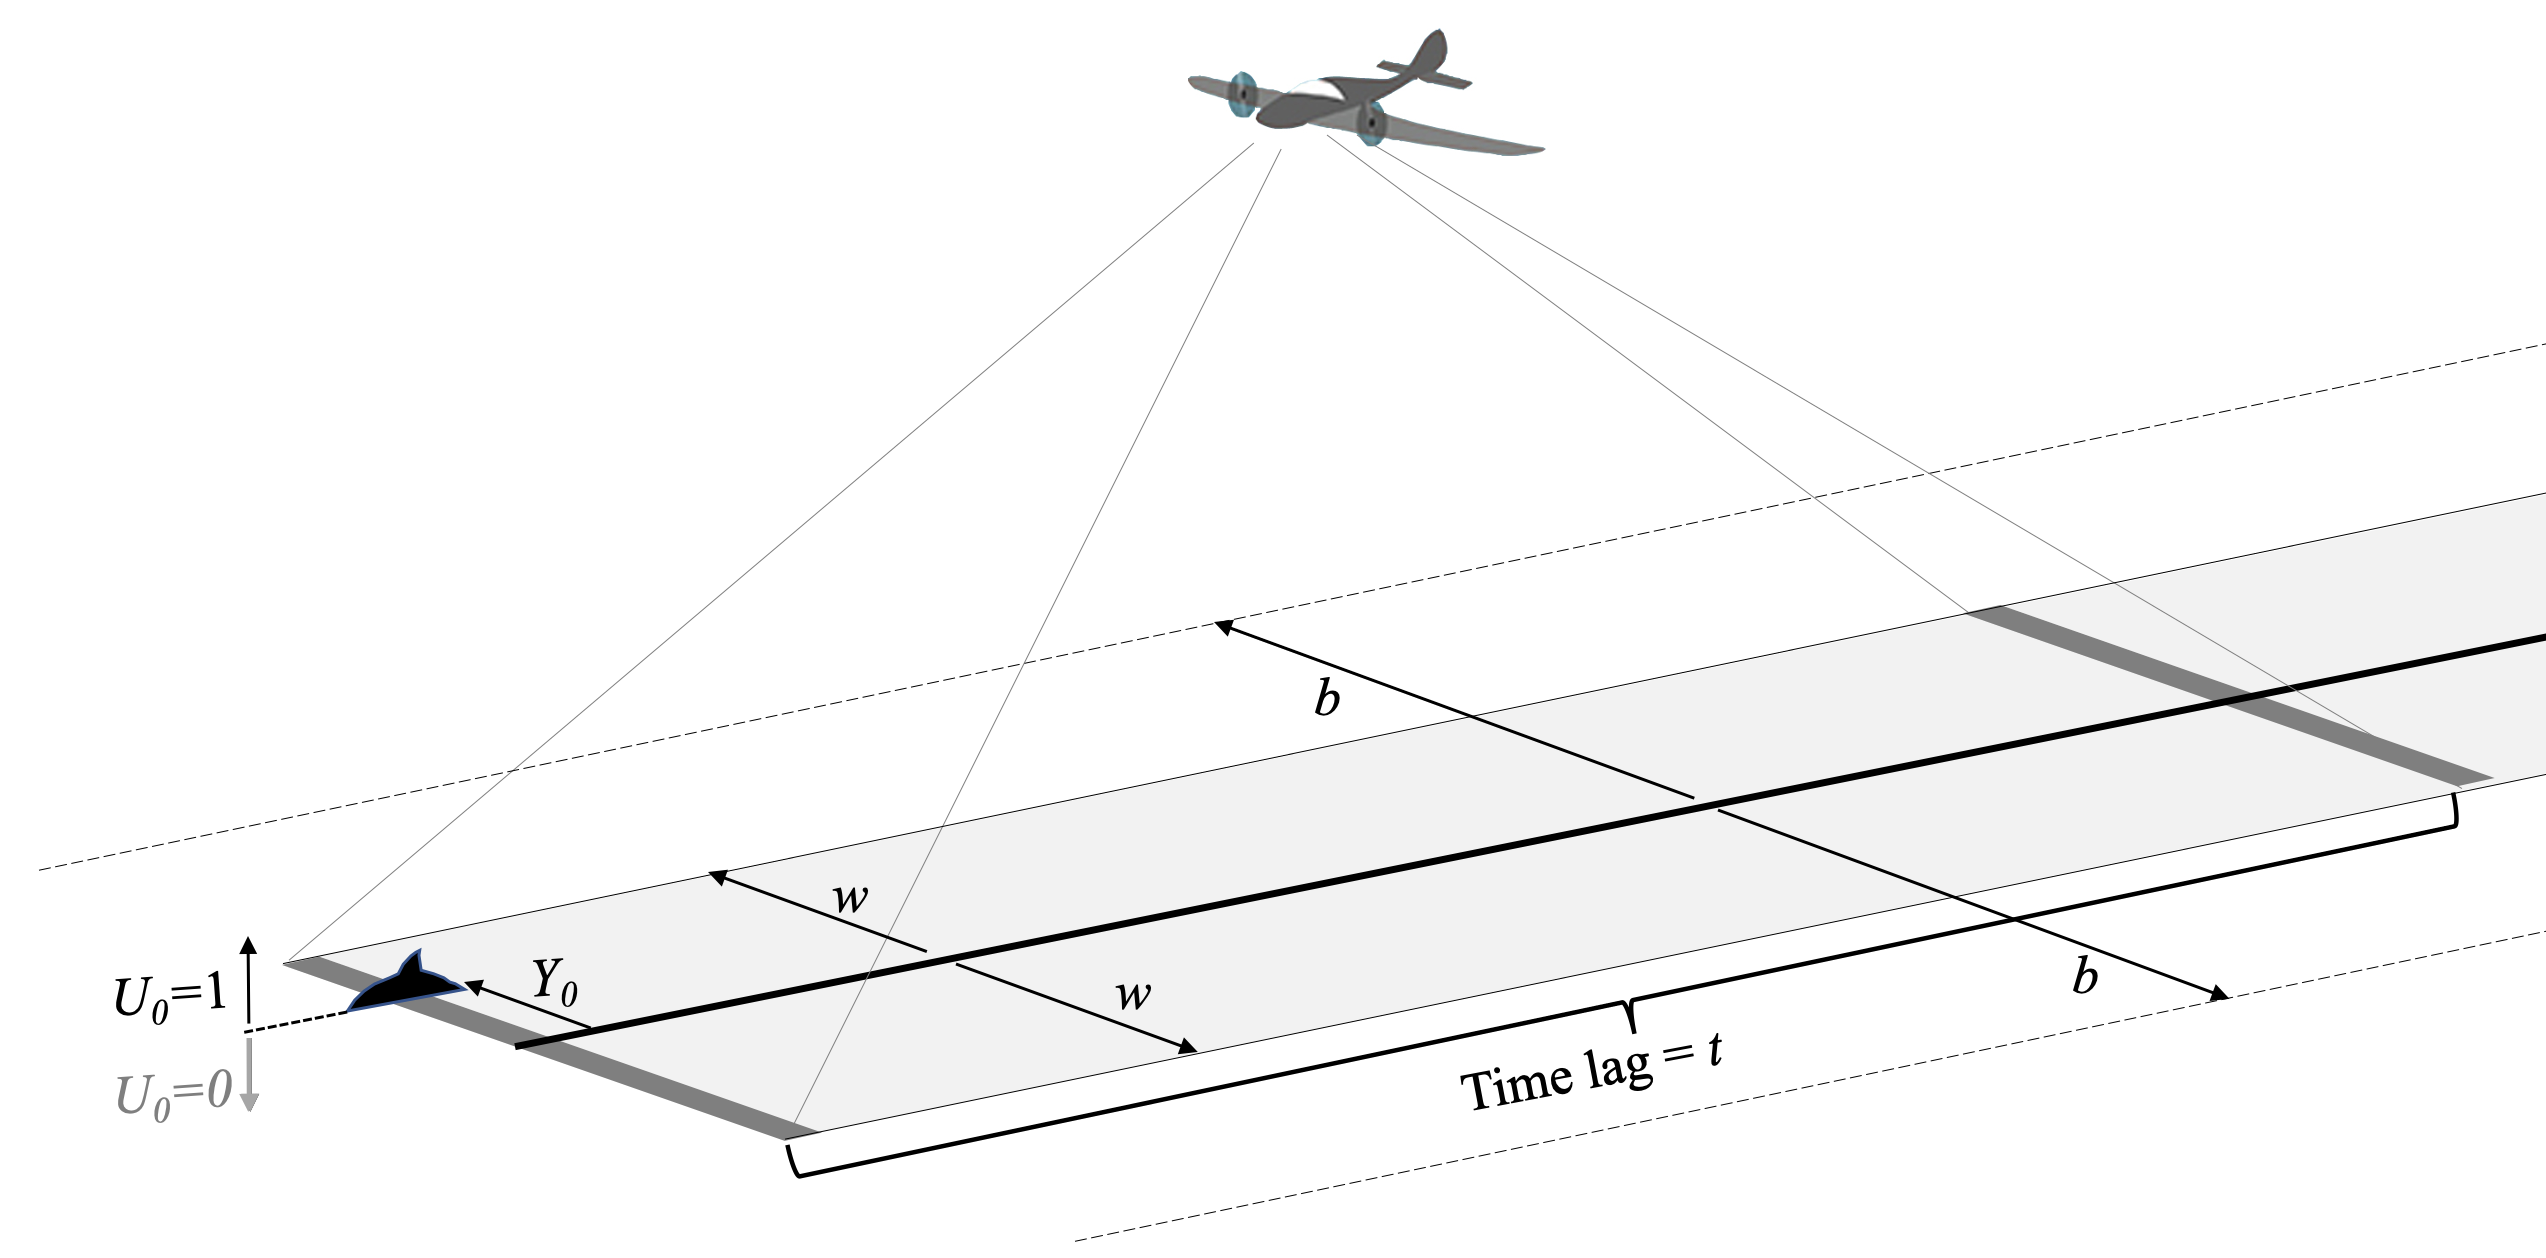
\includegraphics[width=0.75\textwidth]{twocams.png}
\centering
\caption{Illustration of two-camera survey (here with both cameras on a single aircraft). Both cameras survey the grey strip, separated by a time difference $t$. This surveyed strip has half-width $w$. The fields of view of the cameras are indicated by dark grey strips spanning the width of the surveyed strip. It may be possible for animals within a wider strip of half-width $b$, to move into or out of the grey strip between the passing of the first and second camera. $Y_0$ is the distance to the right of the trackline (the dark black centre line), of an animal at the time it comes into the first camera's field of view ($t-0$) and $U_0$ is its availability status at this time ($U_0=1$ if available, $U_0=0$ if not). Its distance and availability at times $t>0$ are $Y_t$ and $U_t$, respectively. Further, the random variable $Z_t$ is defined to be 1 if $|Y_t|\leq w$, and zero otherwise.}
\label{fig:branching_updated}
\end{figure}

We model in/out availability as a two-state Markov process with transition probabilities over an interval of time $t$ given by Eqns~\eqref{eq:p_{IO}} and \eqref{eq:p_{OI}}:
\be
\bm{M}(t)&=&
\left(
\begin{array}{cc}
1-p_{IO}(t) & p_{IO}(t) \\
p_{OI}(t) & 1-p_{OI}(t)
\end{array}
\right)\,.
\label{eq:M}
\ee
The stationary distribution of the in/out Markov chain, which gives the long-term proportion of time spent in each state, is $(w/b, \;1-w/b)$.


%%%RMF - delete this?
%%%There are two reasons that animals that are within the survey strip at some point between the passing of the first and second observers may not be available for detection. The first is that they are invisible to the observers because they are diving. The second is that they are invisible because they are not within the strip at the time they are passed. We construct models for each of these processes below.
%%%

\subsection{Diving behavior and up/down availability}

We model animal diving behavior using a two-state continuous-time Markov chain such that the time spent in state 1 (the near-surface state) is an exponential random variable with expected value $\kappa$, and the time spent in state 2 (the diving state) is an exponential random variable with expected value $\tau-\kappa$, where $\tau$ is the expected dive cycle duration. The Markov transition rate matrix $\bm{Q}$ is
\be
\bm{Q}&=&
\left(
\begin{array}{cc}
-\frac{1}{\kappa} & \frac{1}{\kappa} \\
\frac{1}{\tau-\kappa} & -\frac{1}{\tau-\kappa}
\end{array}
\right) \,.
\label{eq:Q}
\ee
\noindent
The up/down state transition probability matrix at time separation $t$ is $\bm{U}(t)=\exp(\bm{Q}t)$, where $\exp(\;)$ is the matrix exponential function. The stationary distribution of the Markov chain is $(\gamma, \:1-\gamma)$, where $\gamma=\kappa/\tau$.

%\todo[inline]{RMF - put the stationary distribution $\bm{\pi}$ inline, and we don't need a notation for it.}

\subsection{Combined availability model}


The possibilities of being in or out of the detection zone, and up or down with respect to diving, generate four states that animals can occupy: (up and in), (up and out), (down and in), and (down and out). We number the states 1 to 4 in that order. Assuming that the up/down state is independent of the in/out state, the matrix of transition probabilities between these states at time separation $t$ is the Kronecker product $\bm{\Gamma}(t)=\bm{U}(t)\otimes\bm{M}(t)$. Using a matrix formulation for $\bm{\Gamma}(t)$ provides an extendable and computationally efficient way of dealing with the hidden states 2, 3, and 4. The stationary distribution for the four-state Markov process is
\be
\bm{\delta}&=&\Bigg(
\gamma\frac{w}{b},\;
\gamma\left(1-\frac{w}{b}\right),\;
\left(1-\gamma\right)\frac{w}{b},\;
\left(1-\gamma\right)\left(1-\frac{w}{b}\right)
\Bigg).
\label{eq:delta}
\ee



\section{Detection model}

We assume that the probability that an animal is in each state at the time the first observer passes over it is given by the stationary distribution $\bm{\delta}$, and hence that its state distribution after a waiting time $t$, when the second observer passes it, is $\bm{\delta}\bm{\Gamma}(t)$.

Define the binary variable $X_{ij}$ to be 1 if animal $i$ is detected by observer $j$ and zero otherwise. We model $X_{ij}$ as a state-dependent Bernoulli random variable with parameter $p_j(c)=\mbox{Pr}(X_{ij}=1\mid C_{ij}=c)$ where $C_{ij}$ is the state of animal $i$ when observer $j$ passes over it, and $c\in \{1,2,3,4\}$.
It follows that $X_{ij}$ ($j \in \{1, 2\}$) are observations from a Markov modulated Bernoulli process. %\todo[inline]{BCS: Maybe ($j \in \{1, 2\}$) instead?\\ RMF: done -- change made above.}

%\todo[inline]{RMF - no need to define $t_{i1}$ and $t_{i2}$ here. Acronym MMBP never used again so removed.}

% at times $t_{i1}$ and $t_{i2}$. It is convenient to define the time at which the first observer passes animal $i$ ($t_{i1}$) to be zero, so that the time at which the second observer passes is $t_i=t_{i2}-t_{i1}$ ($t$ in the development of the previous section).

It is convenient to arrange the state-dependent probability mass functions of $X_{ij}$ in a diagonal matrix \citep[see][Eqn 2.13]{Zucchini+al:16}. For observer $j$, this matrix is
\be
\bm{P_j}(x_{ij})\;=\;
\begin{blockarray}{cccc}
\text{up,in} & \text{up,out} & \text{down,in} & \text{down,out} \\
\begin{block}{(cccc)}
\text{Bern}(x_{ij};p_j(1)) & 0 & 0 & 0 \\
0 & 1-x_{ij} & 0 & 0 \\
0 & 0 & \text{Bern}(x_{ij};p_j(3)) & 0 \\
0 & 0 & 0 & 1-x_{ij} \\
\end{block}
\end{blockarray}
\ee
\noindent
where $\text{Bern}\big(x_{ij};p_j(c)\big)\equiv p_j(c)^{x_{ij}}\{1-p_j(c)\}^{1-x_{ij}}$. The above matrix allows for animals to be detected in the `down' state, but not in the `out' state. We now assume that $p_j(3)=0$, so that only animals in the `up' state can be detected, but in general this need not be the case.

Let $t_i$ be the time elapsed between the passage of the first and second observers over animal $i$.
Conditional on $t_{i}$, the probability of observing capture history $(x_{i1},x_{i2})$ for animal $i$ can be expressed as the following matrix product, which efficiently sums over hidden states:
\be
\mathbb{P}(x_{i1},x_{i2}\mid t_{i})&=&
\bm{\delta}\bm{P_1}(x_{i1})\bm{\Gamma}(t_{i})\bm{P_2}(x_{i2})\bm{1}\,,
\label{eq:p_omga}
\ee
\noindent
where $\bm{1}$ is a column vector of ones. We label the three observable capture histories as $\dotomega_1=(0, 1)$, $\dotomega_2=(1,0)$, and $\dotomega_3=(1,1)$, and define $q_k(t) = \mathbb{P}(\,\dotomega_k \mid t)$ as given in \eqref{eq:p_omga}. The overall probability of capture history $\dotomega_k$ is then
\begin{equation}
\tilde{q}_k=\mathbb{P}(\,\dotomega_k\,)=E_{t}\left\{ \mathbb{P}(\,\dotomega_k \mid t) \right\}=\displaystyle\int q_{k}(t)f_{T}(t)\,dt\,.
\label{eq:ptilde}
\end{equation}
\noindent

%\todo[inline]{BCS: It's probably that I take a little while to digest equations, but I find the use of $q_k(t)$ a bit confusing and it's not clear why we don't just use $\mathbb{P}(\omega_k \mid t)$. For example, I would have found $\mathbb{P}(\omega_k) = \int_0^\infty \mathbb{P}(\omega_k \mid t) f_T(t) dt$ a bit easier to digest. Is it because using $\tilde{q}_k$ instead declutters Eq (10)?\\
%  RMF: yes, I don't think we can change this, because the $q_k$ notation leads into $\tilde{q}_k$ and $\tilde{q}_\cdot$ and we couldn't replace all these by longhand in later equations. Instead, I've changed the middle terms in the equation above to make the link with $\mathbb{P}(\omega_k \mid t)$ more concrete. Also changed to $\dotomega_k$ in response to Ben's later comment.}


%\todo[inline]{RMF - removed the joint probability statement above, as it isn't needed beyond the expectation; and the $p_{01}(t_i)$ etc notation, which isn't needed and can be confused with transition probabilities. Likewise replaced their only other occurrence in Section 7. Also simplified notation around $\omega$ and $\tilde{p}_k$.}
%The joint probability of the second observer passing animal $i$ at $t_{i}$ and observing $(x_{i1},x_{i2})$ is $p(x_{i1},x_{i2}\mid t_{i})f_{T}(t_{i})$. For brevity, we now write $p(x_{i1}=0,x_{i2}=1\mid t_{i})$ as $p_{01}(t_{i})$, we write $p(x_{i1}=1,x_{i2}=0\mid t_{i})$ as $p_{10}(t_{i})$, and we write $p(x_{i1}=1,x_{i2}=1\mid t_{i})$ as $p_{11}(t_{i})$.


\section{Survey model}

%\todo[inline]{RMF - removed mention of $2bD(s)$, as the meaning of intensity is number per unit area. Simplified likelihood notation and derivation.}

We assume that the number and locations of animals in the forward direction, within distance $b$ of the transect line at the time that the first observer passes overhead, are governed by a Poisson process with intensity $D(s)$ at along-transect location $s$. We derive the likelihood by supposing that the capture history $\omega_i$ of each animal $i$ is known. We will later revoke this requirement by marginalizing over all possible assignments of detections to capture histories.

%As mentioned above, we also assume that animals are uniformly distributed on the interval $(-b,b)$ perpendicular to the transect line, so that the number and location of animals within distance $b$ of the transect follows a Poisson process with intensity $D(s,y)=2bD(s)/2b=D(s)$ at along-transect distance $s$ and perpendicular distance $y\in (-b,b)$ %As a result, points within a distance $b$ of the transect are located in the along-transect dimension according to a Poisson process with intensity $2bD(s)$, where $s$ is the distance along the transect.

Let $\bm{s}=(s_1, \ldots, s_n)$ be the observed forward locations of the $n$ detected animals at the time of first detection. We can write $\bm{s}=\left(\bm{s}^{(1)}, \bm{s}^{(2)}, \bm{s}^{(3)}\right)$ , where $\bm{s}^{(k)}$ corresponds to locations of animals with capture history $\dotomega_k$ for $k=1, 2, 3$. Each set of locations $\bm{s}^{(k)}$ arises from thinning the overall Poisson process by probability $ \tilde{q}_{k}$. Because multinomial splitting of a Poisson process produces independent Poisson subprocesses, the likelihood of $\bm{s}$ is the product of the three likelihoods from the thinned subprocesses. For animals with capture history $\dotomega_3=(1,1)$, there are additional observations on the time delay $t$ between detection by the first and second observers, providing information about the movement parameter $\sigma$. The PDF of waiting time $T$, conditional on the capture history being $\dotomega_3$, is
\be
f_{T \mid \,\omega} (t \mid \dotomega_3) = \frac{f_T(t) \,\mathbb{P}(\dotomega_3 \mid t)}{\mathbb{P}(\dotomega_3)} =  \frac{f_T(t) \,q_3(t)}{\tilde{q}_{3}}\,,
\label{eq:fTgivenOmega}
\ee
where the right-hand side of \eqref{eq:fTgivenOmega} is obtained from Equations~\eqref{eq:fTt}, \eqref{eq:p_omga}, and \eqref{eq:ptilde}. This PDF is included as an auxiliary component to the Poisson process likelihood for $\bm{s}^{(3)}$.

Let $L$ be the total transect length of the survey, and let $n_k$ be the number of observations of capture history $k=1, 2, 3$, with $n_1+n_2+n_3 = n$. Let $\tilde{q}_\cdot=\tilde{q}_1 + \tilde{q}_2 + \tilde{q}_3$ be the overall probability of detection. We write $\bm{s}$, $\bm{\omega}$, and $\bm{t}$ for the locations, capture histories, and (where available) time delays for animals $i=1, \ldots, n$. The parameter vector is $\bm{\theta}$. The likelihood is:
\be
\mathcal{L}(\bm{\theta}\,;\,\bm{s},\bm{\omega}, \bm{t}) = \frac{\exp\left\{ - \int_0^L D(u) \tilde{q}_{\cdot}\,du \,\right\}}{n_1! \,n_2!\, n_3!}
\left\{\prod_{i=1}^n D(s_i) \right\} \tilde{q}_1^{\,n_1}\, \tilde{q}_2^{\,n_2}\,
\prod_{i \,: \, \omega_i=\dotomega_3} \big\{f_T(t_i) \,q_3(t_i) \big\} \,.
\label{eq:LDs}
\ee

%\todo[inline]{BCS: I find the notation for $\omega$ a little confusing. At first we have $\omega_1 = (0, 1), \omega_2 = (0, 1), \omega_3 = (1, 1)$, for example, but later on in Section 5 we say that $\omega_i$ are known for animals $i = 1, \cdots, n$, suggesting that $\omega_1$ is the true capture history for the $i$th individual, not necessarily $(0, 1)$. I'm generally rusty on set notation, but I'm not sure $i \,: \, \omega=\omega_3$ is quite rigorous enough, because $i$ doesn't appear after the colon. If $\omega_i$ is the capture history for the $i$th animal (as defined in Section 5) then I guess we could use $i \, : \, \omega_i = (1, 1)$?\\
%RMF: this distinction between $\omega_i$ and $\omega_3$ has been a perennial problem. I've changed the three fixed capture histories to $\dotomega_k$ throughout using a Latex newcommand \textbackslash dotomega, which can be redefined if David doesn't like it. So now $\omega_i$ ONLY means capture history for animal $i$.}


\subsection{Homogeneous density}

In the homogeneous case, where density is constant throughout the survey, we have $D(s)=D$. The likelihood is:
\be
\mathcal{L}(\bm{\theta}\,;\,\bm{s},\bm{\omega}, \bm{t}) = \frac{\exp\left( - L D \,\tilde{q}_{\cdot}\,\right)}{n_1! \,n_2!\, n_3!} \, D^n\, \tilde{q}_1^{\,n_1}\, \tilde{q}_2^{\,n_2}\,
\prod_{i \,: \, \omega_i=\dotomega_3} \big\{f_T(t_i) \,q_3(t_i) \big\} \,.
\label{eq:LD}
\ee

\subsection{Model parameters}
\label{sec:model_parameters}

The model has four kinds of parameters:

\textbf{Density parameters}: In the case of the homogenous Poisson process there is one parameter, $\theta$, such that $D=e^{\theta}$. When density varies with covariates, $\theta$ is replaced by a linear predictor involving a parameter vector.

\textbf{Dive cycle parameters}: The two-state dive cycle model described above is parametrized in terms of the mean dive cycle length, $\tau$, and the mean proportion of time in the near-surface state, $\gamma$, which are linked to parameters $\alpha_\tau$ and $\alpha_\gamma$ via log and logit links: $\tau=e^{\alpha_\tau}$ and $\gamma=e^{\alpha_\gamma}/(1+e^{\alpha_\gamma})$.

\textbf{Movement parameters}: The animal movement model has one parameter, $\sigma$, which we model using a log link: $\sigma=e^\phi$.

\textbf{Detection parameters}: Assuming that animals are only detectable when in state $c=1$ (up, in), we have two Bernoulli parameters to model: $p_1(1)$ and  $p_2(1)$. These can be modeled using logit link functions. If the observers are identical digital detectors, it may be reasonable to assume these two probabilities are identical, i.e. $p_1(1)=p_2(1)=p=e^\beta/(1+e^\beta)$.

As is the case for density, covariates can be incorporated into the other three models by replacing the corresponding scalar parameter on the link scale with a suitable linear predictor involving the covariates.

%\todo[inline]{RMF - don't need notation $\bm{\theta}^*$.}

For the rest of this paper, we focus on the constant density model with identical detectors and no covariates, which has five parameters: $(\theta,\alpha_\gamma,\alpha_\tau, \phi, \beta)$. \cite{Stevenson+al:19} showed that these are not all identifiable from the two-observer survey design. For the detection model, they assumed that $p=e^\beta/(1+e^\beta)=1$. This is reasonable for digital aerial surveys conducted in calm sea states, if we define the near-surface state to be ``at or breaking the surface'': a state that is easily observed. The field of view of a digital camera is such that objects towards the periphery of the image are as easily detected as objects in the centre of the image, so a detection function that drops off with distance from the line is not needed.

\cite{Stevenson+al:19} also showed that even when $p$ is known, only two of $(\theta,\alpha_\gamma,\alpha_\tau)$ are identifiable, so one of these parameters must be estimated using external data. We follow \cite{Stevenson+al:19} and \cite{Hiby+Lovell:98} and assume that the mean dive cycle duration $\tau=e^{\alpha_\tau}$ is estimated separately, so we treat it as known in the present survey. In what follows, we therefore assume that detection of animals in the up/in state is certain ($p=1$); we use external estimates to set $\tau$; and we estimate the remaining three parameters. These constitute the density, $D$; the mean proportion of time in the near-surface state, $\gamma$; and the movement parameter, $\sigma$. The parameter vector is therefore $\bm{\theta}=(\theta,\alpha_\gamma, \phi)$.

%We do this using the locations along the transect line of detections by the first observer and the locations along the transect line of detections by the second observer (and known observer speed) without assigning capture histories to any individual.

%\todo[inline]{RMF - corrected estimating $\kappa$ to estimating $\gamma$ above. Also removed last sentence which is relevant to the next section.}

\section{Marginalising over the latent capture histories}

The likelihoods \eqref{eq:LDs} and \eqref{eq:LD} are formulated under the supposition that the capture history vector $\bm{\omega}$ is known for animals $i=1, \ldots, n$. However, the core problem when observers are separated in time is that the capture histories cannot be known with certainty: they are latent variables. Here we address this problem by enumerating all plausible combinations of latent capture histories. We marginalize the likelihood by summing over the individual likelihoods for every plausible capture history combination. We refer to each combination of capture histories as a ``pairing'', since once the pairs of detections with capture history $\dotomega_3=(1,1)$ have been decided, the capture histories $(0, 1)$ or $(1, 0)$ of all other detections are determined, because we know which of the two observers made each detection.

Calling the $m$th set of pairings $\bm{\omega}^{(m)}$, and the associated vectors of first-detection locations and time delays  $\bm{s}^{(m)}$ and $\bm{t}^{(m)}$ respectively, we obtain the likelihood for the parameters $\bm{\theta}$ as
%we can consider $\mathcal{L}(\bm{\theta};\bm{s}\mid\bm{\omega}^{(m)}, \bm{t}^{(m)})$ to be the conditional likelihood, given $\bm{\omega}^{(m)}$.
\be
\mathcal{L}(\bm{\theta})&=&\sum_{m=1}^M\mathcal{L}\left(\bm{\theta}; \bm{s}^{(m)},\bm{\omega}^{(m)}, \bm{t}^{(m)}\right)\,,
\ee
\noindent
where $M$ is the number of plausible pairings.


While this likelihood is easy to write down, it is challenging to evaluate because we need to enumerate all $M$ plausible combinations $\bm{\omega}^{(m)}$. For any but very small sample sizes, the number $M$ of possible pairings is very large. We tackle this problem by first partitioning the location vector $\bm{s}$ into subsets between which paired detections are impossible, to reduce the number of plausible pairings, and then using a constraint programming technique for efficient enumeration of all possible pairings within subsets. The constraint programming algorithm is described in Appendix~B.


\subsection{Subdivision of $\bm{s}$}

We partition $\bm{s}$ by ``cutting'' the transect line immediately after detections by observer $j$ for which the distance to the next detection by the other observer is greater than a maximum possible distance that an animal could have moved between the two observers passing over it ($d_{max}$). This distance $d_{max}$ must be decided using knowledge of the movement speed and behavior of the target species. A suitable value for $d_{max}$ can be chosen by doing inference at a range of plausible values to find where estimates become insensitive to $d_{max}$. The cost of setting $d_{max}$ too large is in computational speed; the cost of setting $d_{max}$ too small is positive bias in estimation of $D$, since setting $d_{max}$ too small will result in some animals with true capture history $(1,1)$ being assigned capture history $(0, 1)$ or $(1,0)$.

%\todo[inline]{RMF - changed $C$ and $c$ to $R$ and $r$ below, as $C$ and $c$ are HMM states.}
Having divided the transect line into $R$ segments, we enumerate the possible pairings $\bm{\omega}^{(m_r)}$ for segments $r=1,\ldots,R$. Let $M_r$ be the number of possible pairings in segment $r$. We calculate the likelihood as
\be
\mathcal{L}(\bm{\theta})&=&\prod_{r=1}^R\sum_{m_r=1}^{M_r}\mathcal{L}\left(\bm{\theta};\bm{s}^{(m_r)},\bm{\omega}^{(m_r)},\bm{t}^{(m_r)}\right)\,.
\ee

When $d_{max}$ is substantially smaller than most of the distances between detections by different observers, segmentation can lead to a massive reduction in computation time, making it quite feasible to compute what would otherwise be an intractable likelihood.



\subsection{Interval estimation}
\label{sec:ci}

We estimate the variances of parameters using the inverse of the Hessian obtained in the fitting process. Confidence intervals for the parameters $D$, $\sigma$ and $\gamma$ are gained from the inverse log transformation of confidence intervals for $\theta$ and $\phi$, and the inverse logit transformation of $\alpha_\gamma$, assuming normality of the maximum likelihood estimators of these parameters.


\section{Application \label{sec:applic}}

We use the term `Latent Capture-history Enumeration' method, or LCE, to describe our framework. We  developed this method in anticipation of digital aerial survey data becoming widely used, but, pending the availability of analysis methods such as the LCE method developed here, such data are not yet available. We therefore estimate density from the semi-synthetic data used by \cite{Stevenson+al:19}. These data are taken from an aerial survey of harbor porpoise ({\em Phocoena phocoena}) in the North Sea using human observers, compiled from periods when the aircraft circled back over its transect after a lag of $l=248$ seconds.
%\todo[inline]{BCS: I really should have thought of this before, but the circle-backs were not actually all at 248 s. Instead, the average lag across all circle-backs was 248 s. I just took the average because my CCR code can't deal with different lags for different transects. However, this method can incorporate the different lags more easily can't it? Do we also want to analyse these data with the exact lags, rather than the average lag?\\
%RMF: I vote for not doing any more analyses. We could insert `average', as in, `after an average lag of $l=248$ seconds', but I don't feel we need to make a big deal of this since it's synthetic data anyway. I haven't made any change.}
The two observers correspond to the two passes of the aircraft. Only data in a narrow strip of half-width $w=0.125$ km are included, to mimic the narrow field of view and perfect near-surface detection characteristic of digital observers. As noted by \cite{Stevenson+al:19}, a lag of $l=248$ seconds is longer than any plausible value for $\tau$, and as a consequence the surfacing states of an animal at the times the two observers pass are independent and the estimator is robust to unknown $\tau$. For shorter lags $\tau$ needs to be specified (see Section~\ref{sec:sim}).

%\todo[inline]{RMF - Ben didn't need to specify $\tau$ for this analysis because the two observers were considered independent for such a long lag. How did you deal with this? There hasn't been a previous mention of $\tau$ not being needed if you can assume independence. In some ways this should come after the comments done in Fig 1, but I can see why you want to put the application first; so some sort of comment is needed.\\
%DLB: I set $\tau$ in the estimation code, to be 110 seconds, as in Ben's simulations, but also checked that estimates were insensitive to $\tau$ by estimating with some other values. Added the two sentence at end of paragaph above.}



%\todo[inline]{RMF: I needed to move some text around in the next paragraph to explain what $\sigma_{palm}$ is and refer to Appendix C.}

Following \cite{Stevenson+al:19}, we use a buffer of $b=2$ km, beyond which we assume no animal could enter the detection zone between the passage of the two observers.  \cite{Stevenson+al:19} applied a Palm likelihood estimation approach, termed cluster capture-recapture (CCR).
%\todo{BCS: Have previously defined this acronym. Do we need to do so again? RMF: no harm done by repeat.}
For comparison with their work we quote results for parameter $\sigma_{palm}$ and mean animal speed: see Appendix~C for the relationship between these parameters and the parameter $\sigma$ used above. \cite{Stevenson+al:19} obtained the following estimates, with 95\% confidence intervals in brackets: $\hat{D}=1.05$ (0.84, 1.60) pods per km$^2$; $\hat{\sigma}_{palm}=0.15$ $(0.11, 0.19)$ km; and the expected proportion of time in the surface state, $\hat{\gamma}=0.86$ (0.56, 1.00). Using the LCE method, we obtain $\hat{D}=1.24$ (0.97,1.6) pods per km$^2$, $\hat{\sigma}_{palm}=0.09$ (0.07,0.11) km, and $\hat{\gamma}=0.73$ (0.55,0.91). The estimate $\hat{\sigma}_{palm}=0.09$ corresponds to a mean rate of displacement over $l=248$ seconds of $0.58$ m/s, with 95\% confidence interval ($0.47$,$0.71$) m/s.

\cite{Stevenson+al:19} estimated the coefficients of variation (CV) of $\hat{D}$, $\hat{\sigma}_{palm}$ and $\hat{\gamma}$ to be $19$\%, $16$\%, and $13$\%, respectively. The corresponding estimated CVs from the LCE method are $13$\%, $10$\%, and $13$\%, respectively.

The estimates from the two methods are broadly consistent; the LCE method estimates there to be substantially less animal movement, slightly less time at the surface, and a higher animal density. As we cannot evaluate the relative merits of the methods on the basis of a single survey with unknown density, we investigate their performance by simulation.


\section{Simulation study \label{sec:sim}}

%If detections $X_{i1}$ and $X_{i2}$ of animal $i$ by the two observers were independent, we could estimate detection probability and density using two-sample mark-recapture or mark-recapture distance sampling. The estimated detection probability for either observer would then reflect the probability of the joint event that the animal is available and detected, and the proportion of time spent available would need to be estimated separately. However, in practice it is unlikely that availability of moving and diving animals is independent for the two observers.

%In that case, if $p_1=p_2=1$, then the estimated detection probability from MRDS or two-sample mark-recapture methods would be an estimate of the availability probability, while if $p_j<1$ ($j=1,2$) then it would estimate the product of the probability that an animal is available and $p_j$.

%\todo[inline]{RMF - removed the bit about MRDS and availability. It opens a can of worms, because for MRDS you have simultaneous observers so movement isn't relevant. With LCE, we deliberately introduce a time lag to enable us to estimate availability, but this means we have to create models for movement and diving, AND we still need external data to estimate $\tau$.  So why not just use a single-observer transect (no need for MRDS with digital cameras), and use external data to estimate the proportion of time available, instead? Comparisons with MRDS here might invite the reviewers to ask awkward questions\ldots \\
%DLB: I am OK with this change, although in general it is not true to say that MRDS has simultaneous observers, and that movement isn't relevant (it is true for digital cameras). The reason we do not use single-observer transect methods is that we do not want to have to use external data to estimate the proportion of time available - because these data are typically difficult to get, and the proportion may change from place to place and time to time, so that you may be using the wrong proportion. This difficulty was one of the main reasons for developing our method. Us needing external data for $\tau$ is unfortunate (we did not know we'd need this when starting to develop this method). The density estimate may be less sensitive to misspecification of $\tau$ than the single-observer method is to misspecification of the proportion, but I guess we don't want to invite referees to ask us to look into that.}


Recall that $X_{i1}$ and $X_{i2}$ are detections of animal $i$ by two observers separated by a time lag. With lags close to zero, $X_{i1}$ and $X_{i2}$ are highly correlated because animals available to one observer are almost certain to be available to the other. As lag increases, we expect this correlation to decrease. A pertinent question is whether dependence can be removed by choosing a suitably long lag. To investigate this we look at the correlation between $X_{i1}$ and $X_{i2}$ as a function of lag, with $\gamma$ values from 0.1 to 0.9, and lags from 0 to $500$ seconds.

In our model, $X_{i1}$ and $X_{i2}$ are Bernoulli random variables with expectation $\gamma w/b$. The correlation between these variables when there is a separation of $t$ seconds between the two observers passing over an animal, is
\be
\rho(t)&=&
\frac{
\sum_{x_{i1}=0}^1\sum_{x_{i2}=0}^1
\left(x_{i1}-\gamma\frac{w}{b}\right)\left(x_{i2}-\gamma\frac{w}{b}\right) \mathbb{P}(x_{i1}, x_{i2} \mid t)
}{\gamma\frac{w}{b}\left(1-\gamma\frac{w}{b}\right)}\,,
\ee
\noindent
where $\mathbb{P}(x_{i1}, x_{i2} \mid t)$ is given in \eqref{eq:p_omga}.

%\todo[inline]{RMF - replaced notation $p_{X_1 X_2}$ which I removed from Section 3.}

%The probability of an animal being detected by observer 2 ($X_{i2}=1$), given that observer 1 detected it ($X_{i1}=1$) $t$ seconds earlier, is
%\be
%p(1,1|t_{i})&=&
%(1,0,0,0)\bm{P}(1)\bm{\Gamma}(t)\bm{P}(1)\bm{1}.
%\ee

The dark line in Figure~\ref{fig:fig_correlation_plot} shows the correlation as a function of the lag ($t=l$) for $\tau=110$ seconds and $\gamma$ and $\sigma$ equal to the estimates obtained in the previous section. It also shows the correlation for $\gamma\in\{0.1, 0.2,\ldots,0.9\}$ and the correlation under the assumption that animals do not move but do become unavailable by diving.

\begin{knitrout}
\definecolor{shadecolor}{rgb}{0.969, 0.969, 0.969}\color{fgcolor}\begin{figure}

{\centering 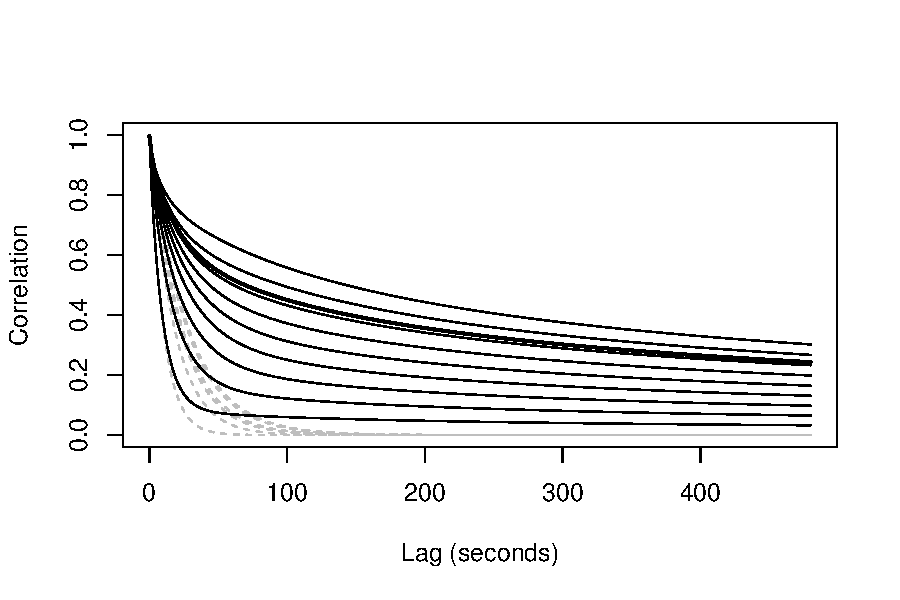
\includegraphics[width=\maxwidth]{figs/fig_correlation_plot-1} 

}

\caption[Correlation between detections by the two observers as a function of lag for mean proportions of time available \(\gamma=10\%\) (bottom black line), \(20\%, 30\%, 40\%, 50\%, 60\%, 70\%, 80\%, 90\%\) (top black line)]{Correlation between detections by the two observers as a function of lag for mean proportions of time available \(\gamma=10\%\) (bottom black line), \(20\%, 30\%, 40\%, 50\%, 60\%, 70\%, 80\%, 90\%\) (top black line). The thick black line is for \(\gamma=73\%\). The grey dashed lines show the correlation under the assumption of no animal movement.}\label{fig:fig_correlation_plot}
\end{figure}


\end{knitrout}

It is clear that increasing the lag to $\tau$ or more reduces correlation to approximately zero if animals do not move (grey lines), although in the presence of animal movement there is still correlation between observers due to in/out availability. The decay to zero corroborates the observation of \cite{Stevenson+al:19} that correlation between observers due to up/down availability can be removed by setting a lag greater than $\tau$. With such long lags, the up/down availability model requires only the single parameter $\gamma$, corresponding to the proportion of time spent at the surface. This has the considerable advantage that there are no unidentifiable parameters, so no external data are needed to estimate density.

% In the presence of animal movement, therefore, we cannot design our way out of the problem of correlated detections by increasing the lag between observers.

%\todo[inline]{RMF - removed the bits about needing a model for availability and can't design ourselves out of correlated detections. If we're talking about lags at all, we already have a model for availability. I thought the real point about a long lag is that we no longer need external data to estimate the extra parameter $\tau$. This links back to the comment in Section 6 about what you did about $\tau$ there? I've made a suggested edit, but this needs to be tidied up more carefully by a comment in Section 6.\\
%DLB: There is received wisdom in MRDS that increasing lag decreases dependence, but no received wisdom that dependence never goes to zero. Hence the sentence seems worthwhile to me. But removing it is OK.}

%\todo[inline]{RMF - The units of $\sigma$ should be metres, not $m/s$, so I'm not sure what is intended here when you say that the $\sigma$ values are equal to speeds and given in $m/s$? Can you fix by saying the $\sigma$ values `correspond to' speeds, rather than `equal' speeds? Also, I removed the $\gamma$ of 10\%, and changed $\sigma=0.5$ to $\sigma=0.65$, to match the values specified in Table 1: please check this is OK.}

In practice, we are primarily interested in methods for surveys with two cameras on one aircraft, and with this configuration and fast-moving aircraft, lags of more than some tens of seconds are unlikely to be achievable. In light of this, and the results of Figure~\ref{fig:fig_correlation_plot}, we present simulations for (a) a scenario designed to imitate the porpoise survey above, and (b) scenarios with lag $l$ of 10, 20, 50 and 80 seconds, and $\gamma$ appoximately equal to, and bracketing, the estimates of $\gamma$ obtained above, namely 0.5, 0.8, and 0.9. For $\sigma$ we use values 15, 8 and 23, which correspond to the rounded mean of the estimated $\sigma_{palm}$ from the LCE and CCR methods (in m), converted from $\sigma_{palm}$ to $\sigma$ (see Appendix C), and to rounded values that are 50\% smaller and 50\% larger, respectively. In all cases, we use the same $\tau$ in estimation as was used in simulation. For the short-lag scenarios in (b), we perform simulations with true density $D=1.24$, as estimated in the previous section, and with an observer speed of 100 knots, which is around the typical speed of marine aerial surveys. We performed 1000 simulations for each scenario.

%\todo[inline]{Need to say how many simulations.}

\subsection{Simulation based on harbor porpoise data: lag of 248 seconds}

%\todo[inline]{RMF - added a sentence about line length: is it correct that you increased the sample size by changing $L$? I've left the value of $L$ to be filled in. BCS: Yep, I've filled it in.}

For this scenario we use the estimates of \cite{Stevenson+al:19} as the generating values, corresponding to $D=1.05$, $\gamma=0.86$ and $\sigma_{palm}=0.15$. Initial line length is $L=1100$ km, which is subsequently doubled or tripled to increase sample sizes. We investigate by simulation the bias and precision of the LCE estimator. In the light of our results in Section \ref{sec:applic}, where we obtained an LCE estimate that was 18\% greater than the CCR estimate of \cite{Stevenson+al:19}, we also investigate whether this discrepancy is within the bounds expected due to estimator variability.

% within what one would expect by chance, or might reflect some bias or model misspecification with one or both of the estimators.



%\todo[inline]{RMF - moved paragraphs around to reflect order of importance.}

For density $D$, the empirical bias and CV of the LCE and CCR estimators from 1000 simulations are $9.9$\% (CV=$29.8$\%) and $12.7$\% (CV=$37.9$\%), respectively. The biases reduce to $4.3$\% (CV=$18.0$\%) and $5.1$\% (CV=$21.4$\%) when sample size is doubled while holding density constant, and to $2.9$\% (CV=$14.6$\%) and $3.3$\% (CV=$16.7$\%) when sample size is tripled.

%\todo[inline]{BCS: Changed from $round(simres$pc.bias.mle,1)$\% (CV=$round(simres$pc.cv.mle,1)$\%) and $round(simres$pc.bias.palm,1)$\% (CV=$round(simres$pc.cv.palm,1)$\%) for original sample size,  3.5\% (CV=20\%) and 4.1\% (CV=23\%) for doubled sample size, and 2.9\% (CV=17\%) and 3.5\%  (CV=18\%) for trebled sample size. I suspect some of the new values are larger because my simulations had $N \sim \text{Poisson}(E(N))$, but perhaps the old ones had $N$ fixed? I think other differences are because the original values only used 150 iterations, but these used 1000. Should I redo with fixed $N$? Can easily be done.}


The correlation between LCE and CCR density estimates from the simulations is $0.75$, while the probability of getting a relative difference as large as, or larger than, that observed is approximately $20$\%, from which we conclude that the observed difference is not large enough to raise concerns about the validity of either estimator with the porpoise data.


%\todo[inline]{RMF: two queries about the next paragraph. \\ Ben: is it true that CCR actually can't do variable encounter times, or just that this hasn't been implemented yet? \\ David: is it correct to change the sentence at the end to `difference between encounter lag and observer lag being only 2.4\% of the observer lag'?}
%\todo[inline]{BCS: I suspect that you might be able to incorporate variable encounter times, but it probably wouldn't be straightforward.\\
%RMF: I looked at the CCR paper and it looks like it should be possible by incorporating an integral over $t$ into the expressions for $P(U_2 | U_1)$ and $P(Z_2 | Z_1)$. I've added `currently' below to indicate that CCR currently does not do this without excluding the possibility that it could.}

The LCE estimator formulates the delay in encounter times between the two observers as a random variable, due to along-transect animal movement towards or away from the second observer, while the CCR method currently does not, and instead assumes these times to be equal to the lag time between the observers. We anticipate that this will cause the expected values of the two estimators to diverge for long lags, or for the case where animal speeds are non-negligible relative to observer speeds, and this may cause the CCR estimator of density to become biased. Here, however, with the observers moving some 50 times faster than the animals, and the standard deviation of the difference between encounter lag and observer lag being only 2.4\% of the observer lag, the effect on the CCR estimator is very small.

\subsection{Short lag scenarios}

%\todo[inline]{RMF: Deleted $\gamma=0.1$ and changed to $\sigma=0.65$ again.  I've left units of $\sigma$ as $m/s$ but presume it should be changed to $m$. Also need to specify $L$, $w$, and $\tau$ for reproducibility.}
%\todo[inline]{BCS: It should be $L = 1100$ km, $w = 0.125$ km, $\tau = 110$. I have added them below.\\
%RMF: Thanks. David, that just leaves the check of $\gamma$ and $\sigma$ values, and units of $\sigma$, to do.}

Here we investigate the bias and confidence interval coverage of the LCE density estimator under short lag scenarios, and compare them with those obtained from the CCR estimator of \cite{Stevenson+al:19}. There are 36 simulation scenarios corresponding to all combinations of lag $l \in \{ 10, 20, 50, 80\}$ seconds,  $\gamma \in\{ 0.5, 0.8, 0.9 \}$, and $\sigma\in\{ 8, 15, 23\}$. We set $L = 1100$ km, $w = 0.125$ km, and $\tau = 110$ s. Simulation results are summarized in Table~\ref{tab:mlesims_bcs}. Boxplots of the LCE density estimates for each of the 36 scenarios are shown in Figure~\ref{fig:fig_boxplots_bcs}.

%***\todo[inline]{RMF - Table 1 has numerous strange rounding errors for $\gamma$, e.g.\ 0.21 instead of 0.2, etc.\\ DLB: This is a problem with making dynamic tables in .Rnw files. Leave to sort once manuscript is complete.}

\begin{knitrout}
\definecolor{shadecolor}{rgb}{0.969, 0.969, 0.969}\color{fgcolor}\begin{figure}

{\centering 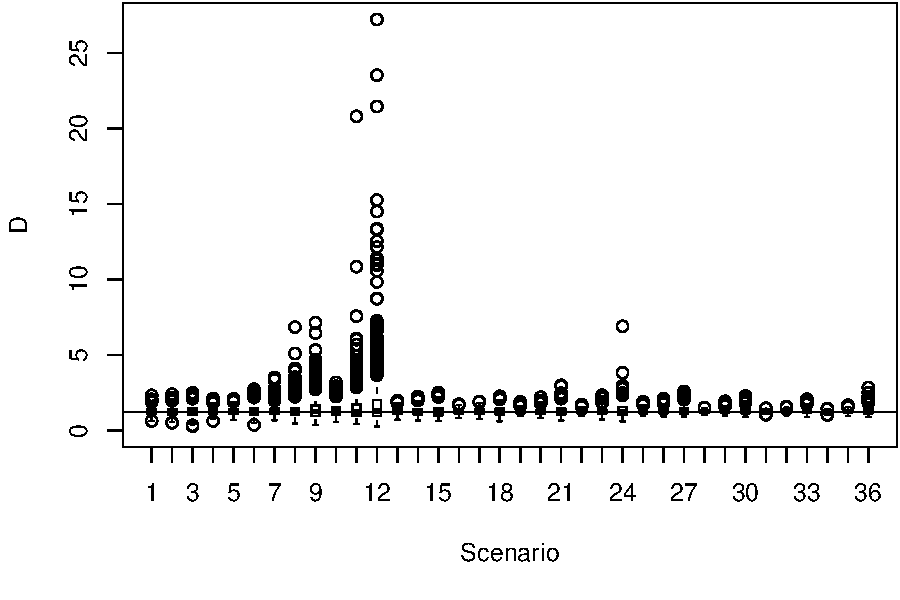
\includegraphics[width=\maxwidth]{figs/fig_boxplots_bcs-1} 

}

\caption[Box plots of estimated LCE density for each of the 36 scenarios]{Box plots of estimated LCE density for each of the 36 scenarios. The horizontal line is at true density \(D=1.24\). }\label{fig:fig_boxplots_bcs}
\end{figure}


\end{knitrout}



% latex table generated in R 3.6.2 by xtable 1.8-4 package
% Sat Jul 25 10:50:54 2020
\begin{table}[ht]
\centering
\caption{Simulation results for LCE and CCR estimators from 1,000 simulations. Here gamma is the proportion of time animals are available, lag is the time between observers, sigma is the animal diffusion rate parameter, mean(n) and mean(m) are the mean numbers of detections by one observer and the mean number of recaptures, across simulations.} 
\label{tab:mlesims_bcs}
\begingroup\setlength{\tabcolsep}{6pt}
\scalebox{0.7}{
\begin{tabular}{rrrrrrrrrrr}
  \hline
 & gamma & lag & sigma & \%BiasLCE & \%cvLCE & \%CoverLCE & \%BiasCCR & \%cvCCR & mean(n) & mean(m) \\ 
  \hline
1 & 0.50 & 10.00 & 8.00 & 2.21 & 16.93 & 0.95 & 1.12 & 20.00 & 170.77 & 132.86 \\ 
  2 & 0.50 & 10.00 & 15.00 & 1.17 & 21.19 & 0.93 & 0.22 & 26.52 & 170.65 & 122.80 \\ 
  3 & 0.50 & 10.00 & 23.00 & 4.30 & 27.56 & 0.90 & 2.15 & 33.57 & 170.74 & 111.29 \\ 
  4 & 0.50 & 20.00 & 8.00 & 1.51 & 12.73 & 0.95 & 0.78 & 14.94 & 170.51 & 111.97 \\ 
  5 & 0.50 & 20.00 & 15.00 & 1.72 & 17.07 & 0.94 & 0.06 & 20.53 & 170.06 & 99.12 \\ 
  6 & 0.50 & 20.00 & 23.00 & 3.36 & 22.38 & 0.93 & 1.98 & 28.00 & 170.85 & 85.25 \\ 
  7 & 0.50 & 50.00 & 8.00 & 1.21 & 10.23 & 0.96 & 0.39 & 11.93 & 170.72 & 81.12 \\ 
  8 & 0.50 & 50.00 & 15.00 & 1.86 & 15.58 & 0.96 & -0.02 & 18.91 & 170.78 & 66.02 \\ 
  9 & 0.50 & 50.00 & 23.00 & 4.95 & 24.10 & 0.94 & 1.92 & 29.16 & 170.46 & 51.06 \\ 
  10 & 0.50 & 80.00 & 8.00 & 1.25 & 10.62 & 0.95 & 0.05 & 12.74 & 170.26 & 69.23 \\ 
  11 & 0.50 & 80.00 & 15.00 & 2.45 & 17.22 & 0.95 & 1.28 & 21.46 & 171.15 & 52.54 \\ 
  12 & 0.50 & 80.00 & 23.00 & 7.90 & 32.99 & 0.92 & 5.33 & 45.14 & 171.08 & 39.22 \\ 
  13 & 0.80 & 10.00 & 8.00 & 2.51 & 11.81 & 0.95 & 3.89 & 15.93 & 273.34 & 229.51 \\ 
  14 & 0.80 & 10.00 & 15.00 & 4.33 & 15.89 & 0.91 & 5.16 & 21.74 & 272.54 & 211.30 \\ 
  15 & 0.80 & 10.00 & 23.00 & 6.94 & 22.44 & 0.86 & 8.78 & 30.79 & 271.98 & 190.81 \\ 
  16 & 0.80 & 20.00 & 8.00 & 1.10 & 7.49 & 0.98 & 0.90 & 9.86 & 272.79 & 209.18 \\ 
  17 & 0.80 & 20.00 & 15.00 & 2.66 & 10.49 & 0.95 & 3.04 & 14.48 & 272.21 & 185.03 \\ 
  18 & 0.80 & 20.00 & 23.00 & 5.29 & 16.63 & 0.93 & 5.15 & 22.17 & 272.47 & 158.80 \\ 
  19 & 0.80 & 50.00 & 8.00 & 0.78 & 5.49 & 0.98 & 0.61 & 7.10 & 273.61 & 181.84 \\ 
  20 & 0.80 & 50.00 & 15.00 & 1.41 & 8.57 & 0.96 & 1.57 & 12.04 & 272.70 & 146.84 \\ 
  21 & 0.80 & 50.00 & 23.00 & 3.25 & 14.52 & 0.95 & 3.40 & 19.64 & 272.12 & 114.33 \\ 
  22 & 0.80 & 80.00 & 8.00 & 0.08 & 5.50 & 0.98 & -0.32 & 7.17 & 271.88 & 168.45 \\ 
  23 & 0.80 & 80.00 & 15.00 & 1.57 & 9.50 & 0.96 & 0.73 & 12.45 & 273.69 & 128.56 \\ 
  24 & 0.80 & 80.00 & 23.00 & 4.74 & 18.09 & 0.92 & 3.46 & 21.25 & 273.04 & 94.71 \\ 
  25 & 0.90 & 10.00 & 8.00 & 2.28 & 7.34 & 0.99 & 3.50 & 11.03 & 306.86 & 264.08 \\ 
  26 & 0.90 & 10.00 & 15.00 & 3.59 & 10.65 & 0.98 & 4.48 & 15.76 & 307.17 & 244.15 \\ 
  27 & 0.90 & 10.00 & 23.00 & 7.58 & 16.88 & 0.95 & 10.36 & 24.91 & 307.25 & 221.46 \\ 
  28 & 0.90 & 20.00 & 8.00 & 0.50 & 4.32 & 0.99 & 0.29 & 5.99 & 306.26 & 247.58 \\ 
  29 & 0.90 & 20.00 & 15.00 & 1.99 & 6.51 & 0.98 & 2.32 & 9.83 & 307.15 & 220.34 \\ 
  30 & 0.90 & 20.00 & 23.00 & 3.53 & 11.57 & 0.96 & 4.61 & 17.10 & 305.50 & 188.14 \\ 
  31 & 0.90 & 50.00 & 8.00 & 0.27 & 4.31 & 0.99 & -0.15 & 5.62 & 306.65 & 226.09 \\ 
  32 & 0.90 & 50.00 & 15.00 & 0.48 & 6.05 & 0.99 & 0.34 & 8.68 & 306.53 & 183.73 \\ 
  33 & 0.90 & 50.00 & 23.00 & 3.02 & 10.29 & 0.95 & 3.23 & 14.00 & 306.43 & 142.15 \\ 
  34 & 0.90 & 80.00 & 8.00 & 0.18 & 4.45 & 0.99 & -0.11 & 5.85 & 306.40 & 212.91 \\ 
  35 & 0.90 & 80.00 & 15.00 & 1.25 & 7.22 & 0.97 & 0.52 & 9.77 & 305.61 & 160.81 \\ 
  36 & 0.90 & 80.00 & 23.00 & 4.23 & 13.94 & 0.90 & 4.72 & 18.11 & 307.35 & 119.72 \\ 
   \hline
\end{tabular}
}
\endgroup
\end{table}




The LCE density estimator is unbiased or nearly unbiased in all 36 scenarios. Figure~\ref{fig:fig_mlepalm_bias_bcs} shows the empirical bias as a function of the mean number of detections by each observer, together with the empirical bias of the CCR estimator fitted to the same simulated data. The bias of the two estimators is very similar. The correlation between the two estimators varies from $0.576$ to $0.871$ across the 36 scenarios, and the mean difference of the estimator means from the true density, as a percentage of the true density, is $2.71\%$ in the case of the LCE estimator, and $1.7\%$ in the case of the CCR estimator.

\begin{knitrout}
\definecolor{shadecolor}{rgb}{0.969, 0.969, 0.969}\color{fgcolor}\begin{figure}

{\centering 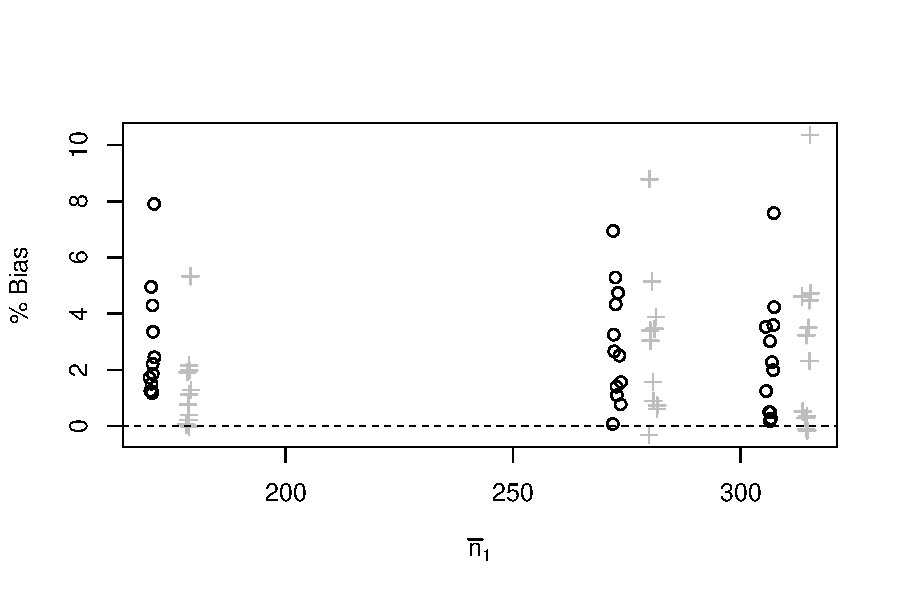
\includegraphics[width=\maxwidth]{figs/fig_mlepalm_bias_bcs-1} 

}

\caption[Percentage difference of estimated density from true density, as a function of mean number of detections by a single observer]{Percentage difference of estimated density from true density, as a function of mean number of detections by a single observer. The LCE estimator is represented by circles, the CCR estimator by crosses. Crosses are offset 8 points to the right, to avoid overlap with circles.}\label{fig:fig_mlepalm_bias_bcs}
\end{figure}


\end{knitrout}



The coefficients of variation of the LCE and CCR density estimators for all 36 scenarios are shown in Figure~\ref{fig:fig_mlepalm_cv_bcs}. The CVs decrease with sample size, as expected. The CV of the LCE estimator is less than that of the CCR estimator in all cases, the more so the larger the sample size. We interpret this to be a consequence of the fact that the CCR estimator is not a maximum likelihood estimator, being based instead on an approximation to the Palm likelihood of pairwise comparisons between detections, so it does not have the asymptotic efficiency of a maximum likelihood estimator. Nevertheless, the difference in precision of the two estimators is very small.

%\todo[inline]{BCS: I don't think this is quite right. It is based on the exact Palm likelihood, not an approximation to the Palm likelihood. However, the Palm likelihood is not the true likelihood. Maybe the middle clause could be changed to ``being based instead on comparing pairwise distances between observed locations''?\\
%RMF: no, the CCR method isn't the exact Palm likelihood.  The approximation step is to use the inhomogeneous Poisson process likelihood instead of whatever the real Palm likelihood is. If we *could* derive the true Palm likelihood, it should be a true likelihood and as efficient as any other. I haven't changed the text above.}


\begin{knitrout}
\definecolor{shadecolor}{rgb}{0.969, 0.969, 0.969}\color{fgcolor}\begin{figure}

{\centering 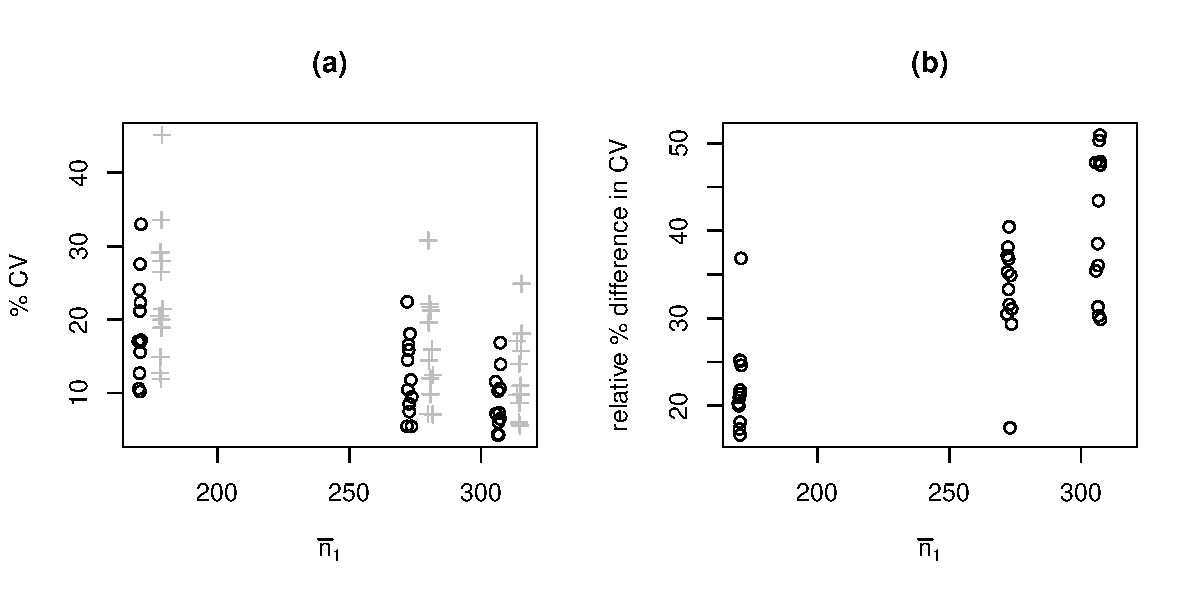
\includegraphics[width=\maxwidth]{figs/fig_mlepalm_cv_bcs-1} 

}

\caption[Percentage coefficient of variation (\%CV), as a function of mean number of detections by a single observer]{Percentage coefficient of variation (\%CV), as a function of mean number of detections by a single observer. The LCE estimator is represented by circles, the CCR estimator by crosses. Crosses are offset 8 units to the right, to avoid overlap with circles. Panel (a) shows the \%CV. Panel (b) shows the amount by which the CV from the CCR method exceeds that from the LCE method, expressed as a percentage of the LCE CV.}\label{fig:fig_mlepalm_cv_bcs}
\end{figure}


\end{knitrout}


In almost all cases coverage probability is close to 95\% (Table~\ref{tab:mlesims_bcs}), with coverage probability tending to be a bit worse when lag is short and there is greater movement (larger $\sigma$), and tending to be too high when animals are almost always avaiable ($\gamma=0.9$). We conclude that for these scenarios, the LCE estimator is approximately unbiased, with confidence interval coverage usually close to nominal, but slightly high when animals are almost always avaiable. The performance of the LCE and CCR estimators is very similar, with the LCE estimator making a slight gain in precision as sample size increases.


\section{Discussion\label{sec:discussion}}

%\todo[inline]{RMF - Not sure the Burt reference is a convincing start to the Discussion here, since we haven't mentioned MRDS previously and we don't have distance in our analysis. Better to launch here with the breadth and potential for extension of the method? This also implies moving the text about identifiable parameters from the end of the Discussion to the beginning. I've put in a possible structure below. Ignore it if you don't like it.}

We have focused here on surveys for diving animals conducted by UAVs, but the LCE method is applicable to a broad range of survey scenarios. In its simplest formulation, our full model involves parameters $D$ and $\sigma$ for modeling density and animal movement, and three parameters for detection and availability: parameter $p$ for detection of available animals, and parameters $\tau$ and $\gamma$ to model availability via the diving cycle. Only one of the three parameters $(p, \tau, \gamma)$ is identifiable from the two-observer design \citep{Stevenson+al:19}, but in many survey scenarios this is not an impediment to application.

For our scenario, involving narrow-strip surveys of diving animals from UAVs, we set $p=1$, obtained $\tau$ from external data, and estimated $\gamma$. For UAV surveys of non-diving animals, including land surveys, the parameters $\tau$ and $\gamma$ are not needed, so parameter $p$ can be estimated from the two-observer data. This survey type is described as mark-recapture or double-count aerial surveys, and the new development offered by LCE is to accommodate animal movement and uncertain capture history into this design. For surveys with a wider field of view, for example from conventional aircraft, detection may decrease with distance from the trackline and the survey type is described as mark-recapture distance-sampling (MRDS). In this case, additional data are collected on the perpendicular distances of animals from the trackline, enabling additional parameters to be estimated which describe the decay of detections with distance. The LCE method provides a framework for MRDS surveys to incorporate animal movement and uncertain capture histories, developments that have been recommended in previous work \citep{Burt+al:14}.

An area for future investigation is whether additional parameters might become identifiable by changes to the survey design, such as operating the survey at a variety of different lags between the two observers, deploying more than two cameras, or adding covariates. In particular, surveying at different lags is a promising and practicable option that might enable the detection parameter $p$ to be estimated along with the availability cycle parameters.

%As was shown by \cite{Stevenson+al:19}, it is not possible to estimate all parameters of interest from two-observer data with unobserved capure histories. However, varying the lag, or having more than two cameras operating may make one more parameter identifiable. It is possible that incorporating covariates into some of the parameters will also make more parameters identifiable. This is an area worth exploring in future.


% \cite{Burt+al:14} note that most MRDS models do not allow for animals to be at different distances from different observers, and say ``A more satisfactory approach would be to develop models that incorporate movement, but this is not straightforward and remains to be done.''. We have done that here, although our detection function is customized for digital aerial surveys, with certain detection within distance $w$ of the transect. If capture histories \textit{are} known, as is assumed with MRDS models, the LCE model provides a framework for extending MRDS aerial survey methods to incorporate animal movement and allow for the fact that the observers commonly observe the same animals at different perpendicular distances.% A complication when such an extension with human observers is that, unlike cameras on aircraft, human observers typically have a wide range of forward distances in view at once, so that animals may be within detection range for very much more than an instant. In this case, one would need to model the observers' detection hazard functions rather than their detection probability functions, as has been done by \cite{Langrock+al:13, Borchers+al:13, Borchers+Langrock:15, Borchers+Cox:16}, for example.



%As noted by \cite{Stevenson+al:19}, if capture histories are known the CCR model can be viewed as a kind of SCR area search model, and the same is true for the LCE model.

%\todo[inline]{RMF - can we delete the paragraph about $M_b$?  It's a bit hard to fit in with the rest of the text. Also it's not really a comment about the LCE model/method, it's a more general comment that a dive-cycle availability model is not the same as $M_b$. If keeping it, a reference to $M_b$ would probably be needed (Otis et al?)  I've commented it out for now.}

%Looking at Figure~\ref{fig:fig_correlation_plot}, one might be tempted to think of the LCE model as a kind of M$_b$ area search spatial capture-recapture model, in which capture probability is elevated by first capture and then decays slowly over time. However this is not quite correct, because capture probability for the second observer changes with time since an animal was available for detection by the first observer, whether or not the first observer detected it.
%End of commented paragraph that you might want to revive.


%In the application we considered above, and in our simulations, the observers were moving much faster than the animals (about 50 m/s compared to around 1 m/s). In this case, $f_T(t)$ is virtually indistinguishable from a normal distribution, but for much slower moving observers $f_T(t)$ becomes quite skewed and one needs to take account of the fact that the time between observers passing an animal may be substantially different from the time lag $l$ between observers. The LCE method is able to do this; the CCR method is currently not able to.

The LCE method has some advantages over the CCR method, but its computation time does not scale well as density increases.
%\todo[inline]{BCS: Would it be clearer to say ``computation time does not scale well as density increases''? Otherwise ``does not scale well'' might be a bit difficult to interpret.\\ RMF: Yes: added above.}
While we were able to deal with moderately large sample sizes above, this is because density was low enough that the transect line could be divided into many segments with relatively few possible combinations of capture histories within each segment. The number of possible capture histories increases very rapidly when each observer detects more than a few animals within a segment, and computation by the LCE method will be infeasible in this case. The number of possible capture histories is
\be
N_{CH}&=&\sum_{m=0}^{n_2^*}{n_2^*\choose m}{{}^{n_1^*}\!P_{m}},
\ee
\noindent
where $n_1^*$ is the larger of $n_1$ and $n_2$, and $n_2^*$ is the smaller. For $n_1=n_2=2,\ldots 10$, $N_{CH}$ is 7; 34; 209; 1,546; 13,327; 130,922; 1,441,729; 17,572,114; 234,662,231. As $n_1^*$ increases, the LCE estimation method will become too slow to be practically useful on typical desktop computers. The CCR method, by contrast, scales well and is able to deal with much larger numbers of detections.

%\todo[inline]{RMF: Below, changed CCR not able to accommodate varying encounter times, to doesn't currently accommodate them.}

Being a maximum likelihood method, the LCE method has the advantage of being able to use the extensive inference results and machinery associated with maximum likelihood, including asymptotic efficiency and likelihood-based variance estimators and model-selection criteria such as AIC. The CCR estimator is slightly less efficient than the LCE estimator for large sample sizes, requires variance estimation by bootstrap, and cannot take advantage of likelihood-based model selection tools. It does not currently accommodate varying times between encounters of animals due to animal movement, although in the scenarios we considered this has negligible effect. Finally, the LCE method provides an inference framework that allows inclusion of covariates in all parameters mentioned in Section~\ref{sec:model_parameters}. While covariates were not available for our application, we anticipate that they may be collected on future surveys. It is not clear how easy it would be for the CCR framework to include covariates that change continuously along the transect line, although it should easily accommodate covariates that are constant within, but different along, sections of transect.

%\todo[inline]{RMF - I didn't quite understand the comment about a strict identification algorithm reducing sample size if $p=1$: it seems if $p=1$ then you have to detect all available animals so you can't afford to lose any from a stricter ID algorithm?  Some changes suggested below.}

The major advantage of both the LCE and the CCR frameworks is that they do not require duplicate sightings to be identified between the two observers. We anticipate that this will facilitate substantial reduction in the cost of processing double-observer data, because it allows the estimation process to be automated. For automatic processing we only need an adequate automatic identifier of the target species in each of the two separate video streams. Since false positives are not handled by our framework, criteria for automated object identification must be set conservatively so that the false-positive rate is reduced almost to zero. This will have the effect of lowering the detection probability, $p$, so we will not be able to assume that $p=1$. As described above, $p$ is estimable from the data if there is no dive-cycle model, and potentially estimable even in the presence of a dive-cycle model if a varying-lag design is employed. It is therefore likely that fully-automated survey processing will become achievable in the near future, commensurate with advances in object identification algorithms and UAV engineering.


%If false negatives affect only the availability process (e.g. remove animals underwater and partially visible), the only cost of using a strict identification criterion in order to avoid false positives, is reduced sample size. If, however, false negatives affect the detection process (e.g. remove some individuals because although they were as available as possible, a wave broke over them as the observer passed) then the assumption of $p=1$ may be violated and bias may ensue if lag between observers is short. Surveying at different lags may allow estimation of $p$ (in additon to $D$, $\sigma$ and $\kappa$) so that it will likely be possible to automate inference from digital surveys by using automated object identification criteria that are sufficiently strict so as to reduce the probability of false positives to virtually zero, providing that the survey involves effort and detections at more than one lag.



\appendix
%\appendixpage

\section{A. Derivation of $f_{T}(t)$}
\label{appx:firstpassage}

%\todo[inline]{RMF - I've made several edits to tidy up the derivation here.}
Define the time and forward coordinate at which observer 1 passes over an animal to be 0. The animal's forward coordinate at time $t$ is $\sigma W_t$, where $W_t$ is a one-dimensional Brownian motion. The forward coordinate of observer 2 at time $t$ is $-vl+vt$. The time at which observer 2 passes over the animal is therefore the minimum $t$ such that
\be
-vl+vt&=&\sigma W_t \nonumber \\
\Rightarrow \;\;\;\frac{vt}{\sigma} - W_t &=& \frac{vl}{\sigma}\,.
\ee
\noindent
The passage time for observer 2 is therefore $T=\inf\{t: vt/\sigma + B_t = vl/\sigma\}$, where $B_t=-W_t$ is also a Brownian motion. We use the following standard result for the first passage time of a Brownian motion with drift. Suppose a particle follows Brownian motion with drift parameter $c$, such that its location at time $t$ is $X_t=ct+B_t$. The random variable $T=\inf\{t: X_t=a\}$ is the first passage time to location $a$, which has probability density function
\begin{equation}
f_{T} (t) = \frac{ a \exp \Big\{ \frac{- (a-ct)^2}{2t} \Big\} }{\sqrt{2 \pi t^3}}\,.
\end{equation}
\noindent
Substituting $c=v/\sigma$ and $a=vl/\sigma$, we obtain the probability density of the time $T$ at which observer 2 passes over the animal:
\be
f_{T} (t)
&=&
\frac{vl \exp \Big\{ \frac{- v^2(l-t)^2}{2\sigma^2t} \Big\} }{\sqrt{2 \pi\sigma^2 t^3}}\,.
\ee

%\todo[inline]{Note to self: need to simplify this - see Rachel's suggestions.}

%One can view the poblem of finding the pdf of the time between the first and second observers passing an animal as a the problem of finding the first passage time to a point at distance $vl$ from the origin, of a particle following Brownian motion starting at the origin, with constant drift velocity $v$ and diffusion parameter $\sigma$. We can write the process as $Y_t=\sigma B_t+vt$, where $B$ is a Brownian motion and $Y_t$ is the animal's displacement at time $t$.

%\todo[inline]{Currently this is based on these two pages: https://math.stackexchange.com/questions/1053294/density-of-first-hitting-time-of-brownian-motion-with-drift and https://math.stackexchange.com/questions/179210/derivation-of-wiener-process-first-passage-times-using-probability-generating-fu}

%We use the result \textbf{(citation)} that for $X_t=B_t+ct$, where $B$ is a Brownian motion, a ``boundary'' at $a>0$, and a constant drift rate $c\in\mathbb{R}$, the pdf of $T=\inf\{t: X_t=a\}$ is
%\begin{equation}
%f_{T} (t) = \frac{ a \exp \Big\{ \frac{- (a-ct)^2}{2t} \Big\} }{\sqrt{2 \pi t^3}}.
%\end{equation}

%In our case, we have the ``boundary'' (the second observer) at a distance $vl$ from the starting position of the animal, approaching it at speed $v$, and the animal moving according to brownian motion with parameter $\sigma$, so that $Y_t=\sigma B_t+vt$. If we rescale distance to be in units of $\sigma$, i.e. $X_t=Y_t/\sigma$, we have $X_t=B_t+\frac{v}{\sigma}t$ and $a=vl/\sigma$. Hence the pdf of time to the second observer passing, given that the second observer passes a fixed point at a time $l$ later than the first, is
%\be
%f_{T} (t)
%&=&
%\frac{\frac{vl}{\sigma} \exp \Big\{ \frac{- (vl/\sigma-vt/\sigma)^2}{2t} \Big\} }{\sqrt{2 \pi t^3}}
%\;=\;
%\frac{vl \exp \Big\{ \frac{- v^2(l-t)^2}{2\sigma^2t} \Big\} }{\sqrt{2 \pi\sigma^2 t^3}}.
%\ee


\vspace{-12pt}

\section{B. Constraint programming for enumerating all $\bm{\omega}^{(m)}$}
\label{appx:constrprog}

For efficient enumeration of the possible pairings within one segment, we define a simple constraint satisfaction problem (CSP)~\cite[Chapter 6]{russell-norvig-aima3}. A CSP is a triple \(\mathcal{P}=\langle \mathcal{X}, \mathcal{D}, \mathcal{C} \rangle\).  The CSP \(\mathcal{P}\) has a set of decision variables \(\mathcal{X}\), each of which has a set of possible values that it may take, called its \textit{domain}, where \(\mathcal{D}(x)\) is the domain of \(x \in \mathcal{X}\). In addition there is a set of constraints \(\mathcal{C}\) that restrict the combinations of values that may be taken by the variables. A constraint \(c\in \mathcal{C}\) is a relation defined on a set of variables: \(\mathrm{scope}(c)\subseteq \mathcal{X}\). A \textit{solution} is an assignment of values to variables such that each variable is assigned a value from its domain, and all constraints are satisfied.

We define a CSP for a segment as follows. Two detections by different observers may be paired if and only if the distance between them is less than or equal to \(d_{max}\). For each set \(\{i,j\}\) of two observations that may be paired, we define one decision variable \(x_{i,j}\) with domain \(\{0,1\}\). Variable \(x_{i,j}\) is equal to 1 in a solution if and only if the two observations are paired.

Suppose we have two distinct sets, \(s_1=\{i,j\}\) and \(s_2=\{k,l\}\), where  \(i\) may be paired with \(j\), and \(k\) may be paired with \(l\), but the two sets are not disjoint: in other words \(s_1 \cap s_2 \ne \emptyset\). The two sets cannot both be paired simultaneously because they share an observation. In all such cases we add the constraint \((x_{i,j}=0 \vee x_{k,l}=0)\) to prevent such pairing.

We use a backtracking search procedure with forward checking~\cite[Chapter 6]{russell-norvig-aima3} to enumerate all solutions to the CSP. The set of solutions to the CSP corresponds one-to-one to the set of valid pairings within the segment. When a solution is found, the part of the likelihood pertaining to that pairing is calculated, avoiding the need to store the set of pairings and allowing efficient calculation of $\sum_{m_r=1}^{M_r}\mathcal{L}\left(\bm{\theta};\bm{s}^{(m_r)},\bm{\omega}^{(m_r)},\bm{t}^{(m_r)}\right)$.

\section{C. The relationship between $\sigma_{palm}$, $\sigma$ and mean animal speed}
\label{appx:sigmaspd}

The $\sigma$ of \cite{Stevenson+al:19}, which we call $\sigma_{palm}$ here, is based on the displacement of animals from the midpoint of their two locations after time $l$ has elapsed, which is normally distributed with mean zero and variance equal to $\sigma_{palm}^2$. If we let the signed distance between the first and second location be $Y$, then $Y/2\sim N(0,\sigma_{palm}^2)$ and hence $\sqrt{\{Y/(2\sigma_{palm})\}^2}=|Y|/(2\sigma_{palm})\sim\chi(1)$. Using the fact that the expected value of a $\chi(1)$ random variable is $\sqrt{2}/\Gamma(0.5)$, we have that $E\left\{|Y|/(2\sigma_{palm})\right\}=\sqrt{2}/\Gamma(0.5)$, and hence $2\sigma_{palm}=E(|Y|)\Gamma(0.5)/\sqrt{2}$.

The distance $Y$ between the initial location and the location after $l$ seconds, of an animal following Brownian motion with rate parameter $\sigma$, has distribution $Y\sim N(0,\sigma^2l)$, so that $E\left\{|Y|/(\sigma\sqrt{l})\right\}=\sqrt{2}/\Gamma(0.5)$ and $\sigma\sqrt{l}=E(|Y|)\Gamma(0.5)/\sqrt{2}$, and hence $\sigma=2\sigma_{palm}/\sqrt{l}$.

As the average speed of an animal over a period of $l$ seconds is $E(|Y|)/l$, the average speed over $l$ seconds of an animal following Brownian motion with rate parameter $\sigma$ can be written as $\sigma\sqrt{2}/\{\Gamma(0.5)\sqrt{l}\}$.

%\todo[inline]{RMF - removed $E(v)$ above as we use $v$ for the constant speed of the observers. Corrected bracket convention (here and throughout) to $[\{( )\}]$.}

%\todo[inline]{Mostly notes to myself - should trim/remove later.}

%We're considering 1-dimensional movement here. Let $X(t)$ be the location of the animal relative to its starting position after time $t$. Then, assuming it starts at $X(0)=0$, $X(t)\sim N(0,\sigma^2 t)$ and $Z_t=X(t)/(\sigma\sqrt{t})\sim N(0,1)$. Let $U(t)=\sqrt{Z_t^2}$. Then\footnote{See \texttt{https://math.stackexchange.com/questions/1059938/whats-the-expectation-of-square-root-of-chi-square-variable}} $U(t)\sim\chi(1)$. And since the expected value of a $\chi(n)$ random variable is $\sqrt{2}\Gamma((n-1)/2)/\Gamma(1/2)$, $E[U(t)]=\sqrt{2}\Gamma(1)/\Gamma(1/2)=0.7978846$.

%Let  $v(t)=\sqrt{X(t)^2}/t$ be the speed of movement away from the initial postion, at time $t$. then $E(v(t))=E(\sqrt{X(t)^2}/t)=E(\sqrt{Z_t^2}\sigma\sqrt{t}/t)$$=0.7978846\times\sigma/\sqrt{t}$. If we want to model Brownian animal movement in which animals have an average speed of $v(t)$ at time $t$, we need $\sigma=v(t)\sqrt{t}/0.7978846$. For example, to model animal movement with average speed of 0.95m/s, as in \cite{Stevenson+al:19}, at time $t$, we require $\sigma=0.95/0.7978846\sqrt{t}$ m/s, or $0.95/797.8846\approx 0.00119\sqrt{t}$ km/s. With a lag of 248 seconds, this is $\sigma\approx 0.00119\sqrt{248}=0.01874$ km/s, while with a lag of 20 seconds it is $\sigma\approx 0.00119\sqrt{20}=0.00532$ km/s.

%This seems a weird way of calculating $\sigma$, because we would like $\sigma$ to be a property of the animals, and not depend on the time lag is between the first and second observers passing over them! It would be better to assume that the standard deviation of $X(t)$ is proportional to $t$, so that $X(t)\sim N(0,\sigma^2 t^2)$ instead. In this case, $E(v(t))=0.7978846\times\sigma$, which does not depend on $t$.

%\cite{Hiby+Lovell:98} model movement using a gamma distribution. They say (p. 1282) ``\textit{The displacement in pod position over the interval $t$ was assumed to follow a gamma distribution, i.e.,}
%\be
%r(t)\sim\frac{e^{-r/(t\beta)}(t\beta)^{-\alpha}r^{\alpha-1}}{\Gamma(\alpha)}.
%\ee
%\noindent
%\textit{As the scale parameter was made proportional to the interval $t$, the standard deviation of the displacement, rather than its variance, increased in proportion to the elapsed time. We thus assumed continuous movement in one direction, as would result from the pod transiting or moving with a water current rather than a milling movement with frequent changes in direction over $t$.}''

%If we have $X(t)\sim N(0,\sigma^2 t)$, we should have $\sigma=v/0.7978846$, where $v$ is the expected animal movement speed (e.g. for $v=9.5$ m/s, we have $\sigma=9.5/0.7978846\approx 11.9$ m/s, or 0.0119 km/s). This results in a speed  of movement away from the initial postion after 1 second, of 9.5 m/s, reducing with $t$ in inverse proportion to $\sqrt{t}$.


\section*{Acknowledgements}
This work was part-funded by the Royal Society of New Zealand through Marsden grant UOA-1418, the Leverhulme grant ``Statistical models for digital wildlife surveys'' and the EPSRC IAA grant ``High Definition digital aerial survey software''. Stephen Marsland contributed substantially to obtaining the correct expression for $f_T(t)$.

\bibliographystyle{biom}
\bibliography{dlb}

%\newpage
%\section*{Online supplementary material}


\end{document}

